\documentclass[11pt]{article}
\usepackage[letterpaper,margin=0.82in]{geometry}
\usepackage[T1]{fontenc}
\usepackage[utf8]{inputenc}
\usepackage{lmodern,microtype}
\usepackage{amsmath,amssymb,amsthm,mathtools}
\usepackage{graphicx,booktabs,longtable,tabularx,array,multicol}
\usepackage[dvipsnames]{xcolor}
\usepackage{enumitem}
\usepackage{fancyhdr}
\usepackage{hyperref}
\usepackage{listings}
\usepackage{float}
\usepackage[section]{placeins}
\usepackage{caption}
\usepackage{subcaption}
\usepackage{tikz}
\usetikzlibrary{arrows.meta,positioning,shapes.misc}

\definecolor{Ink}{HTML}{17202A}
\definecolor{Muted}{HTML}{566573}
\definecolor{Paper}{HTML}{FAFAF7}
\definecolor{Blue}{HTML}{2E86AB}
\definecolor{Teal}{HTML}{2A9D8F}
\definecolor{Orange}{HTML}{F4A261}
\definecolor{Magenta}{HTML}{A23E8C}
\definecolor{Red}{HTML}{E76F51}
\definecolor{PaleBlue}{HTML}{E6F0F4}
\definecolor{PaleTeal}{HTML}{E6F3F1}
\definecolor{PaleOrange}{HTML}{FBF0E6}
\definecolor{PaleMagenta}{HTML}{F4EAF1}

\color{Ink}
\hypersetup{
  colorlinks=true,
  linkcolor=Blue,
  urlcolor=Blue,
  pdftitle={Projector-Resolved Large Algebraic Signal Model},
  pdfauthor={Komorebi P.},
  pdfsubject={Exact multi-atlas coordinates, Bayesian operator programs, residual-driven refinement, memory, and active planning},
  pdfcreator={},pdfproducer={}
}
\graphicspath{{figures/}}
\pagestyle{fancy}
\fancyhf{}
\renewcommand{\headrulewidth}{0.3pt}
\fancyhead[L]{\small\color{Muted} Projector-Resolved Large Algebraic Signal Model}
\fancyhead[R]{\small\color{Muted} Komorebi P.}
\fancyfoot[C]{\thepage}
\setlength{\parindent}{0pt}
\setlength{\parskip}{5pt}
\setlength{\emergencystretch}{3em}
\setlist[itemize]{leftmargin=1.4em,itemsep=2pt,topsep=3pt}
\setlist[enumerate]{leftmargin=1.7em,itemsep=3pt,topsep=3pt}
\newcolumntype{Y}{>{\raggedright\arraybackslash}X}
\newcolumntype{L}[1]{>{\raggedright\arraybackslash}p{#1}}

\newtheorem{definition}{Definition}[section]
\newtheorem{theorem}[definition]{Theorem}
\newtheorem{proposition}[definition]{Proposition}
\newtheorem{corollary}[definition]{Corollary}
\newtheorem{lemma}[definition]{Lemma}
\newtheorem{conjecture}[definition]{Conjecture}
\theoremstyle{remark}
\newtheorem{remark}[definition]{Remark}
\newtheorem{example}[definition]{Example}
\newtheorem{boundary}[definition]{Boundary}
\newtheorem{certificate}[definition]{Finite certificate}

\DeclareMathOperator{\diag}{diag}
\DeclareMathOperator{\Tr}{Tr}
\DeclareMathOperator{\Var}{Var}
\DeclareMathOperator{\Cov}{Cov}
\DeclareMathOperator{\softmax}{softmax}
\newcommand{\R}{\mathbb R}
\newcommand{\C}{\mathbb C}
\newcommand{\Acal}{\mathcal A}
\newcommand{\Scal}{\mathcal S}
\newcommand{\Pcal}{\mathcal P}
\newcommand{\Gcal}{\mathcal G}
\newcommand{\Mcal}{\mathcal M}
\newcommand{\Tcal}{\mathcal T}
\newcommand{\Fcal}{\mathcal F}
\newcommand{\Ecal}{\mathcal E}
\newcommand{\norm}[1]{\left\lVert#1\right\rVert}
\newcommand{\inner}[2]{\left\langle#1,#2\right\rangle}

\lstset{
  basicstyle=\ttfamily\footnotesize,
  frame=single,
  breaklines=true,
  showstringspaces=false,
  columns=fullflexible,
  backgroundcolor=\color{Paper},
  keywordstyle=\color{Blue}\bfseries,
  commentstyle=\color{Muted},
  stringstyle=\color{Magenta}
}

\newcommand{\StatusBox}[1]{%
\begin{center}
\fcolorbox{Teal}{PaleTeal}{\parbox{0.92\linewidth}{\small #1}}
\end{center}}

\begin{document}

\begin{titlepage}
\thispagestyle{empty}
\begin{tikzpicture}[remember picture,overlay]
\fill[Blue!8] (current page.south west) rectangle (current page.north east);
\fill[Teal!14] ([xshift=-2.25in]current page.north east) rectangle (current page.north east);
\draw[Blue,line width=4pt] ([xshift=.60in,yshift=-.65in]current page.north west)--([xshift=-.60in,yshift=-.65in]current page.north east);
\draw[Magenta,line width=2pt] ([xshift=.60in,yshift=.65in]current page.south west)--([xshift=-.60in,yshift=.65in]current page.south east);
\end{tikzpicture}
\vspace*{1.0in}
{\large\color{Blue}\bfseries PROJECTOR-RESOLVED SEED CALCULUS: CAPSTONE MODEL\par}
\vspace{0.25in}
{\fontsize{31}{35}\selectfont\bfseries Projector-Resolved\\[3pt]Large Algebraic Signal Model\par}
\vspace{0.18in}
{\fontsize{17}{21}\selectfont\color{Muted} Exact Multi-Atlas Coordinates, Bayesian Operator Programs, Residual-Driven Refinement, Memory, and Active Planning\par}
\vspace{0.55in}
\begin{minipage}{0.80\linewidth}
\large
A signal-native world model in which spatial, Fourier, wavelet, polyphase, and categorical coordinates coexist inside one exact reconstruction system, while learned operator programs remain typed, probabilistic, and auditable.
\end{minipage}
\vfill
{\Large\bfseries Komorebi P.\par}
\vspace{0.45in}
\end{titlepage}

\begin{abstract}
This paper presents the Projector-Resolved Large Algebraic Signal Model (PR-LASM), a finite, executable world-model architecture built from exact projector decompositions, coordinate transport, polyphase refinement, operator programs, Bayesian evidence, residual-driven adaptation, memory packets, and active planning.  Each observation is retained in a complete multi-atlas archive consisting of spatial, unitary Fourier, orthonormal Haar, two-dimensional polyphase, and categorical color coordinates.  These atlases are not concatenated informally: their weighted direct sum is proved to be a finite tight frame with an explicit canonical synthesis map.  The model then forms deterministic interpretable features and nested macro, meso, and micro states for statistical prediction without confusing those compressed states with the exact archive.

The learned dynamics are a posterior over a typed finite grammar containing linear, quadratic, action-bilinear, delayed, power-memory, exponential-memory, phase-conditioned, gated, and hybrid programs.  A normal-inverse-gamma regression is fitted inside every program, and predictive evidence is combined with explicit complexity and mechanism penalties.  Exact deterministic replay transitions are stored in a state-action graph; the planner combines known graph outcomes, replay probes, posterior progress, win and loss probabilities, novelty, information value, role statistics, and loop penalties.

The release contains exact reconstruction tests, adaptive mixed-depth packet-tree synthesis, controlled program-identification benchmarks, deterministic interactive planning tests, a static audit of twenty-five supplied local environments, a reproducible Python package, and offline run scripts.  All thirty-six automated tests pass.  On seven controlled algebraic systems, the intended operator family and intended atlas are identified in every case.  The median state-prediction RMSE relative to a single linear portfolio baseline is $0.2393$.  Four deterministic interactive systems are solved.  No official benchmark score or claim of general intelligence is made.
\end{abstract}

\StatusBox{\textbf{Status.}  The exact finite coordinate and reconstruction theorems, program definitions, Bayesian formulas, graph algorithms, and supplied tests are complete under the hypotheses written here.  The controlled benchmarks verify the implementation of the declared mechanisms.  The twenty-five bundled environment trees are statically validated, but they were not executed with the official local runtime in the present build environment.}

\tableofcontents
\clearpage

\section{The final construction problem}

The technical series developed seeds, projectors, transfer blocks, nonlinear interactions, polyphase refinement, special functions, stochastic and quantum realizations, computational packet algorithms, arithmetic packets, and local-to-global completion.  The remaining engineering question is whether those ingredients can be assembled into one coherent model of a changing signal world.

A conventional predictor usually commits early to one representation.  A vector model receives coordinates that have already forgotten geometry.  A convolutional model privileges translation-local structure.  A Fourier model privileges global frequency.  A wavelet model privileges scale and location.  A graph model privileges relational neighborhoods.  None of these choices is wrong, but no single one is uniformly natural.

PR-LASM keeps several exact coordinate atlases simultaneously.  It then lets the posterior decide which atlas, resolution, operator family, and memory mechanism best explain the observed transitions.  The exact frame remains recoverable regardless of that choice.

\begin{figure}[H]
\centering
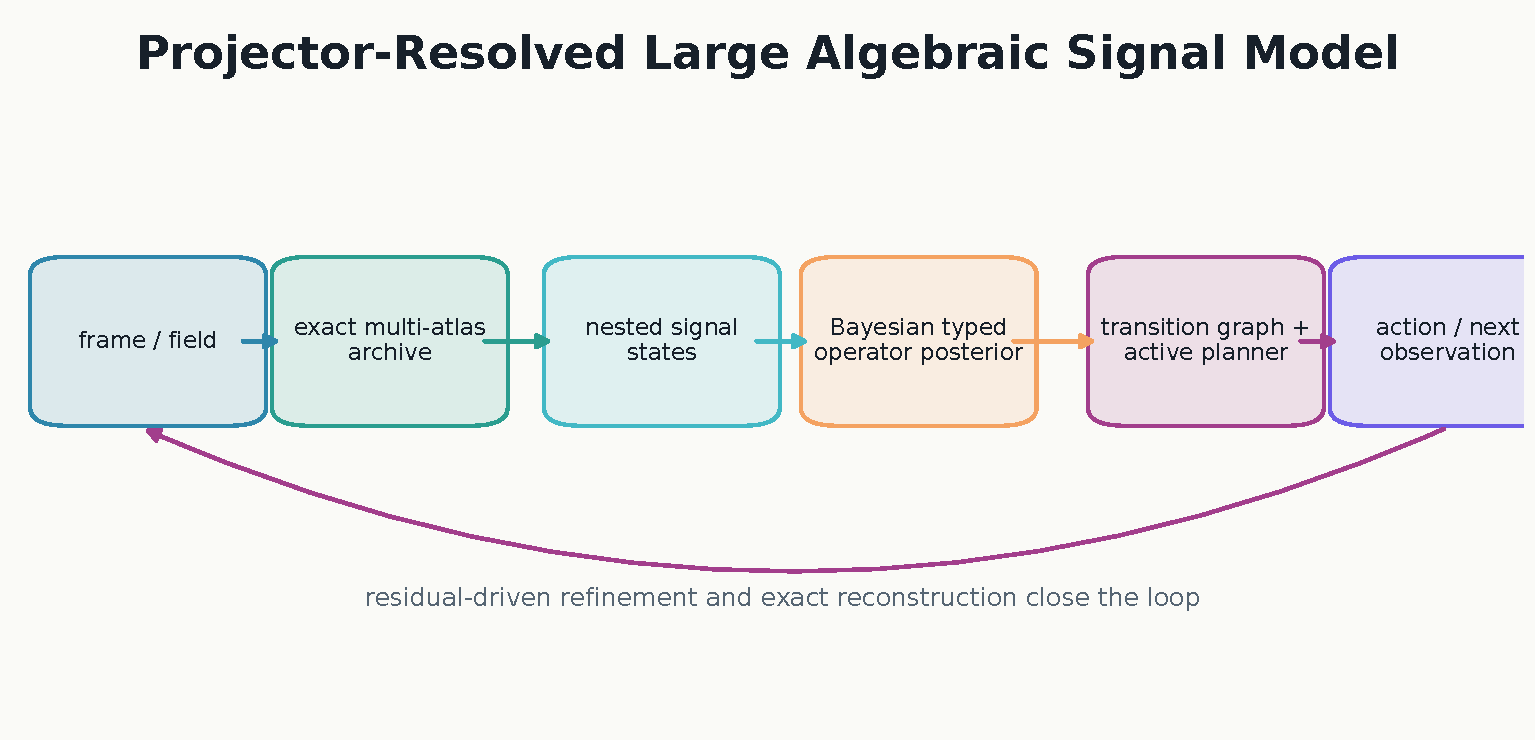
\includegraphics[width=.98\linewidth]{01_pr_lasm_architecture.pdf}
\caption{The completed PR-LASM architecture.  Exact analysis, statistical inference, graph memory, active planning, and reconstruction form one loop.}
\end{figure}

\subsection{What ``large'' means}

The word \emph{large} does not refer only to parameter count.  The model is large because it maintains a structured family of possibilities:
\[
\boxed{
\text{atlas}\times\text{resolution}\times\text{operator program}
\times\text{memory}\times\text{packet refinement}\times\text{action}.}
\]
A small number of parameters inside many typed alternatives can express more structural uncertainty than one dense map with the same total coefficient count.  The model is algebraic because every alternative has an explicit coordinate map, feature map, operator design, probability, and reconstruction status.

\subsection{The strongest defensible claim}

The architecture is a complete candidate for a projector-resolved, exact-reconstruction, multi-atlas, fully algebraic large signal model.  ``Complete'' here means that the finite architecture closes its own declared loop: observation, exact analysis, compression, inference, memory, planning, action, residual measurement, refinement, and reconstruction.  It does not mean that the operator grammar contains every possible law of nature or that the planner solves every interactive environment.

\section{The PR-LASM object}

\begin{definition}[Projector-resolved large signal model]
A finite PR-LASM instance is a tuple
\[
\mathfrak L=
(X,\mathfrak U,\mathfrak E,\mathfrak P,\mathfrak Z,
\mathfrak G,\mathfrak B,\mathfrak H,\mathfrak R,\mathfrak C),
\]
where:
\begin{enumerate}
\item $X$ is the observation space;
\item $\mathfrak U=\{U_a\}_{a\in A}$ is a family of exact coordinate atlases;
\item $\mathfrak E=\{E_{a,\alpha}\}$ is the family of coordinate selectors;
\item $\mathfrak P=\{P_{a,\alpha}\}$ is the pulled-back projector family;
\item $\mathfrak Z$ is a nested family of statistical states;
\item $\mathfrak G$ is a typed operator-program grammar;
\item $\mathfrak B$ is the Bayesian posterior over programs and parameters;
\item $\mathfrak H$ is the explicit memory state;
\item $\mathfrak R$ is the state-action transition graph;
\item $\mathfrak C$ is the planning and reconstruction contract.
\end{enumerate}
\end{definition}

The tuple separates exact coordinates from learned states.  This is not merely editorial.  It prevents a low prediction error in a compressed state from being reported as exact object reconstruction.

\begin{figure}[H]
\centering
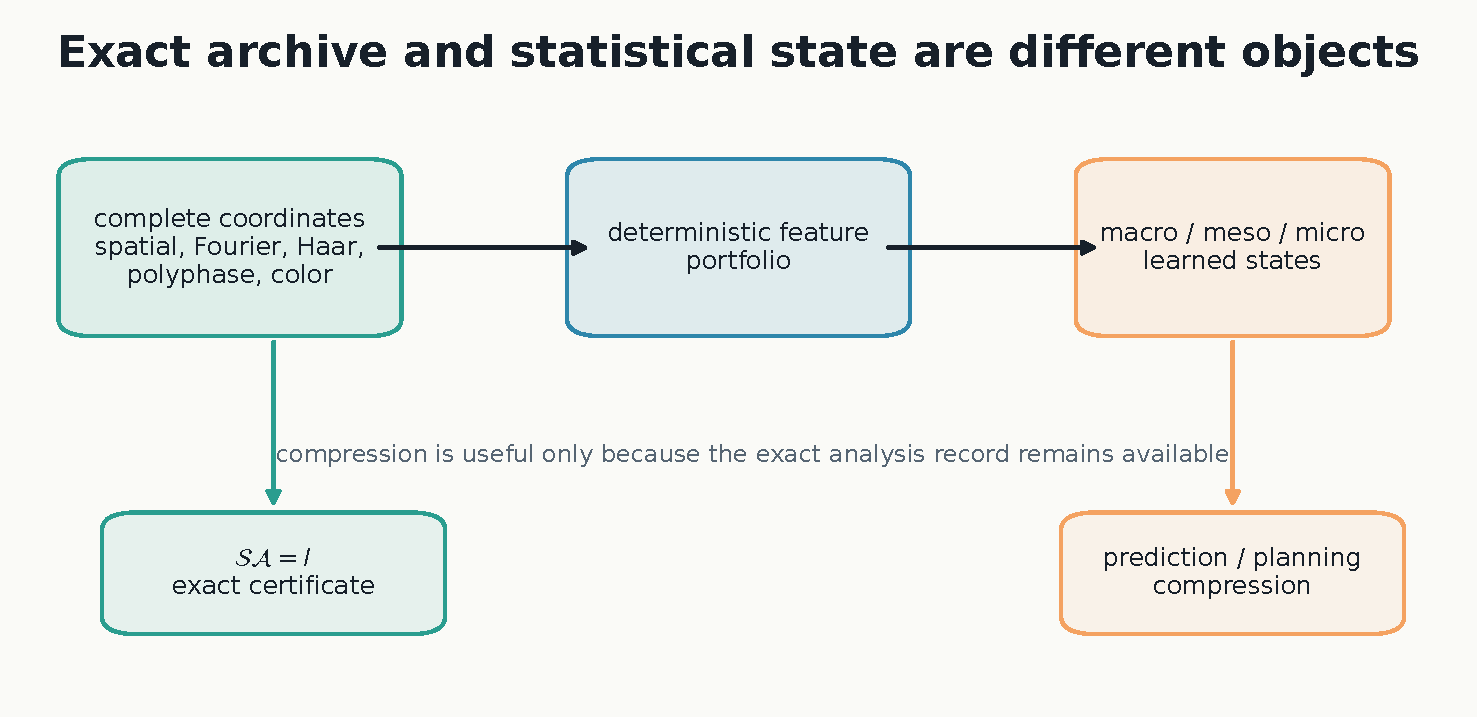
\includegraphics[width=.96\linewidth]{02_exact_archive_vs_statistical_state.pdf}
\caption{The exact coordinate archive and the statistical state serve different purposes.}
\end{figure}

\section{Exact multi-atlas coordinates}

Let $X$ be a finite-dimensional Hilbert space.  For every atlas $a\in A$, let
\[
U_a:X\to Y_a
\]
be unitary, and let $\{E_{a,\alpha}\}_{\alpha\in I_a}$ be orthogonal coordinate projectors satisfying
\[
E_{a,\alpha}E_{a,\beta}=\delta_{\alpha\beta}E_{a,\alpha},
\qquad
\sum_{\alpha\in I_a}E_{a,\alpha}=I_{Y_a}.
\]
Define the object-space packets
\[
\boxed{P_{a,\alpha}=U_a^*E_{a,\alpha}U_a.}
\]

\begin{theorem}[Per-atlas packet reconstruction]
For every atlas $a$, the operators $P_{a,\alpha}$ are orthogonal projectors and
\[
\sum_{\alpha\in I_a}P_{a,\alpha}=I_X.
\]
Consequently,
\[
x=\sum_{\alpha}P_{a,\alpha}x,
\qquad
T=\sum_{\alpha,\beta}P_{a,\beta}TP_{a,\alpha}.
\]
\end{theorem}

\begin{proof}
Conjugation by a unitary operator preserves multiplication, adjoints, and sums.  Therefore
\[
P_{a,\alpha}P_{a,\beta}
=U_a^*E_{a,\alpha}E_{a,\beta}U_a
=\delta_{\alpha\beta}P_{a,\alpha},
\]
and the complete sum is $U_a^*I_{Y_a}U_a=I_X$.  Inserting that identity on one or both sides gives object and operator reconstruction.
\end{proof}

\subsection{A redundant tight-frame atlas}

Choose weights $w_a>0$ and define
\[
\Acal x=(w_aU_ax)_{a\in A},
\]
with synthesis
\[
\Scal(c_a)_{a\in A}
=
\frac{1}{c}
\sum_{a\in A}w_aU_a^*c_a,
\qquad
c=\sum_{a\in A}w_a^2.
\]

\begin{theorem}[Exact multi-atlas tight-frame reconstruction]
The analysis and synthesis maps satisfy
\[
\boxed{\Scal\Acal=I_X.}
\]
Moreover,
\[
\norm{\Acal x}^2=c\norm{x}^2.
\]
\end{theorem}

\begin{proof}
By unitarity,
\[
\Scal\Acal x
=\frac{1}{c}\sum_a w_aU_a^*(w_aU_ax)
=\frac{1}{c}\sum_aw_a^2x=x.
\]
Similarly,
\[
\norm{\Acal x}^2
=\sum_aw_a^2\norm{U_ax}^2
=c\norm{x}^2.
\]
\end{proof}

\begin{figure}[H]
\centering
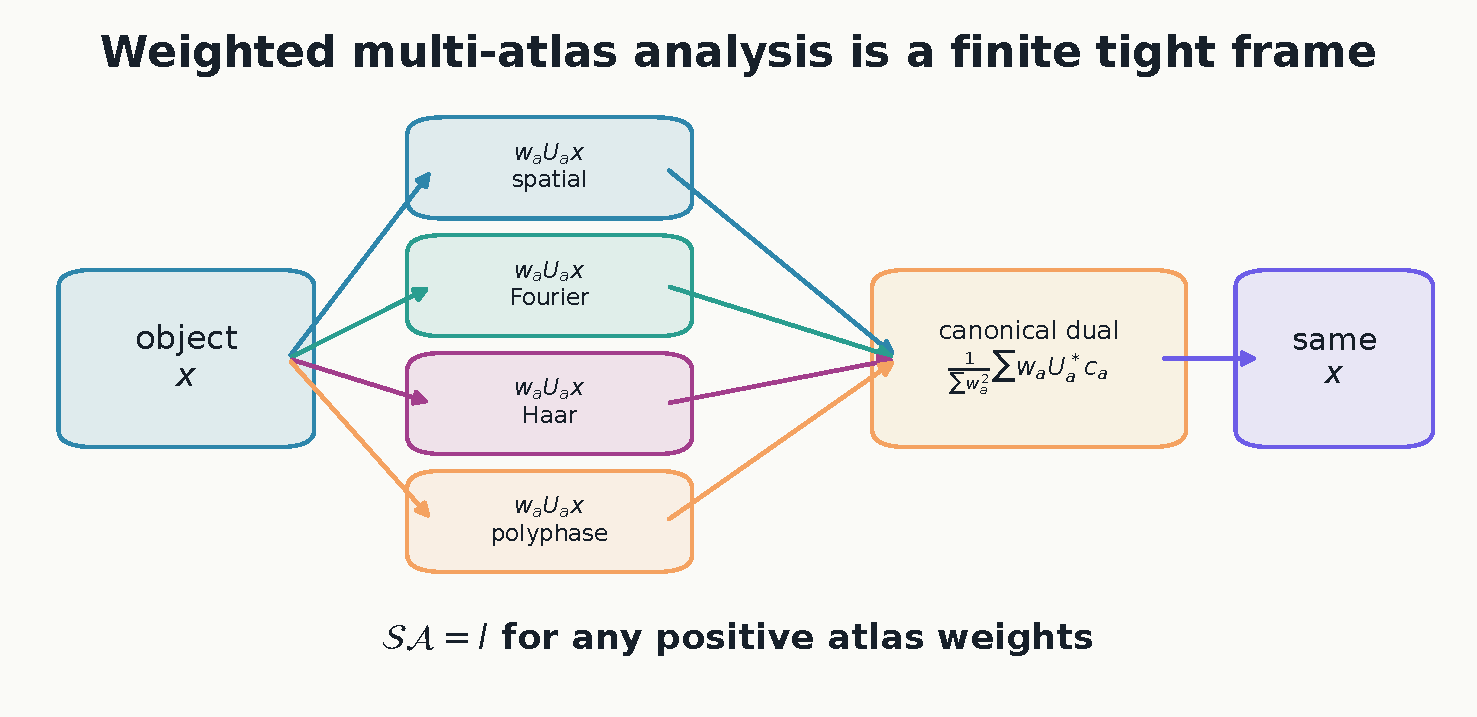
\includegraphics[width=.96\linewidth]{03_multi_atlas_tight_frame.pdf}
\caption{The canonical dual averages exact reconstructions with the correct frame normalization.}
\end{figure}

The normalized positive packets
\[
\widetilde P_{a,\alpha}
=\frac{w_a^2}{c}P_{a,\alpha}
\]
satisfy
\[
\sum_{a,\alpha}\widetilde P_{a,\alpha}=I_X.
\]
They need not be mutually annihilating across different atlases.  They are frame packets, not one enlarged orthogonal projector family.  This distinction prevents the simultaneous use of several atlases from being mistaken for a direct-sum decomposition inside the original space.

\section{Concrete coordinate atlases}

\subsection{Spatial coordinates}

The identity atlas stores the observation itself.  It is the natural chart for local geometry, connected components, boundaries, coordinates, and direct pixel or field values.

\begin{figure}[H]
\centering
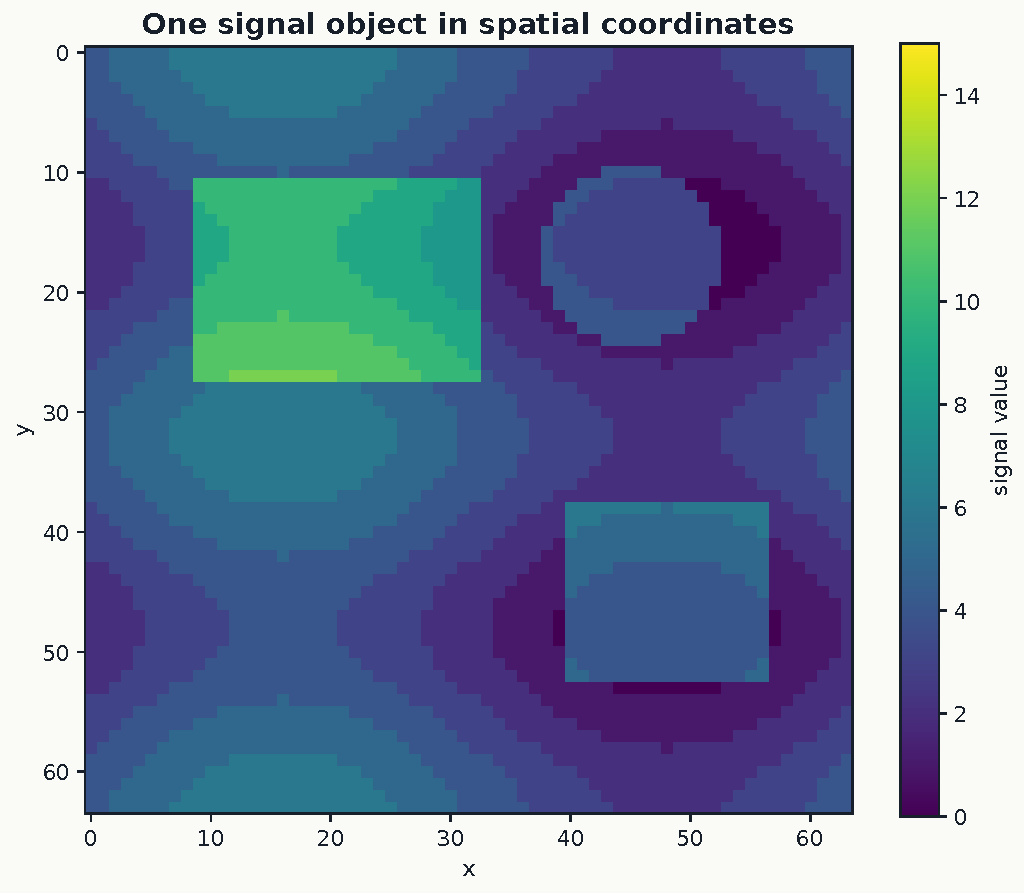
\includegraphics[width=.68\linewidth]{04_sample_signal.pdf}
\caption{A sample finite signal in its spatial chart.}
\end{figure}

\subsection{Fourier coordinates}

For an $H\times W$ array, the normalized two-dimensional transform is
\[
(Fx)_{k,\ell}
=\frac{1}{\sqrt{HW}}
\sum_{m=0}^{H-1}\sum_{n=0}^{W-1}
 x_{m,n}e^{-2\pi i(km/H+\ell n/W)}.
\]
The inverse is $F^*$.  Disjoint frequency masks $E_B$ produce projectors
\[
P_B=F^*E_BF.
\]
Fourier space therefore appears inside the same packet language as any other unitary atlas.

\begin{figure}[H]
\centering
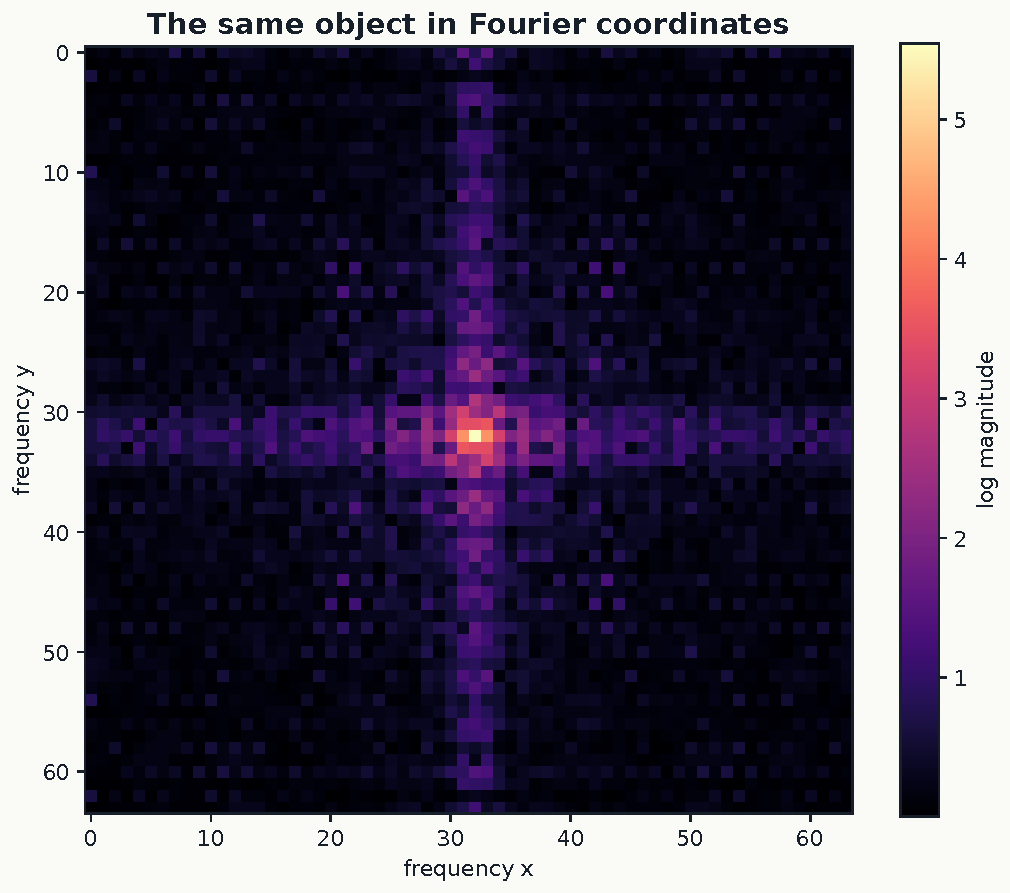
\includegraphics[width=.68\linewidth]{05_fourier_coordinates.pdf}
\caption{Global oscillatory structure becomes visible in Fourier coordinates.}
\end{figure}

\subsection{Haar-wavelet coordinates}

The separable Haar transform repeatedly applies
\[
(a,b)\longmapsto
\left(\frac{a+b}{\sqrt2},\frac{a-b}{\sqrt2}\right)
\]
along columns and rows.  The inverse reverses those operations.  Scale-location selectors in the packed transform pull back to exact wavelet projectors.

\begin{figure}[H]
\centering
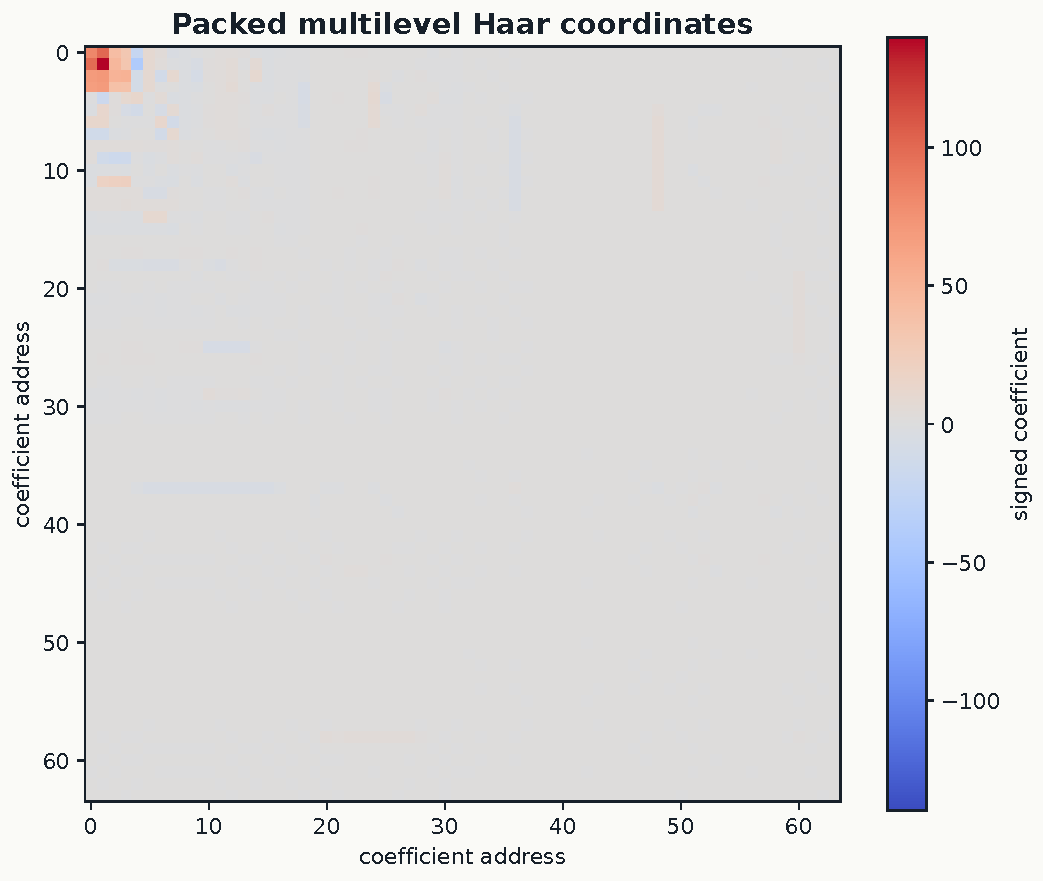
\includegraphics[width=.68\linewidth]{06_haar_coordinates.pdf}
\caption{The same object in a multilevel wavelet chart.}
\end{figure}

\subsection{Two-dimensional polyphase coordinates}

For modulus $N$, define
\[
x_{r,s}[q,t]=x[Nq+r,Nt+s],
\qquad 0\le r,s<N.
\]
The complete channel family is exactly inverted by interleaving.  In object space, the phase projector is
\[
(P_{N,r,s}x)[m,n]
=
\mathbf 1_{m\equiv r\ (N)}
\mathbf 1_{n\equiv s\ (N)}x[m,n].
\]

\begin{figure}[H]
\centering
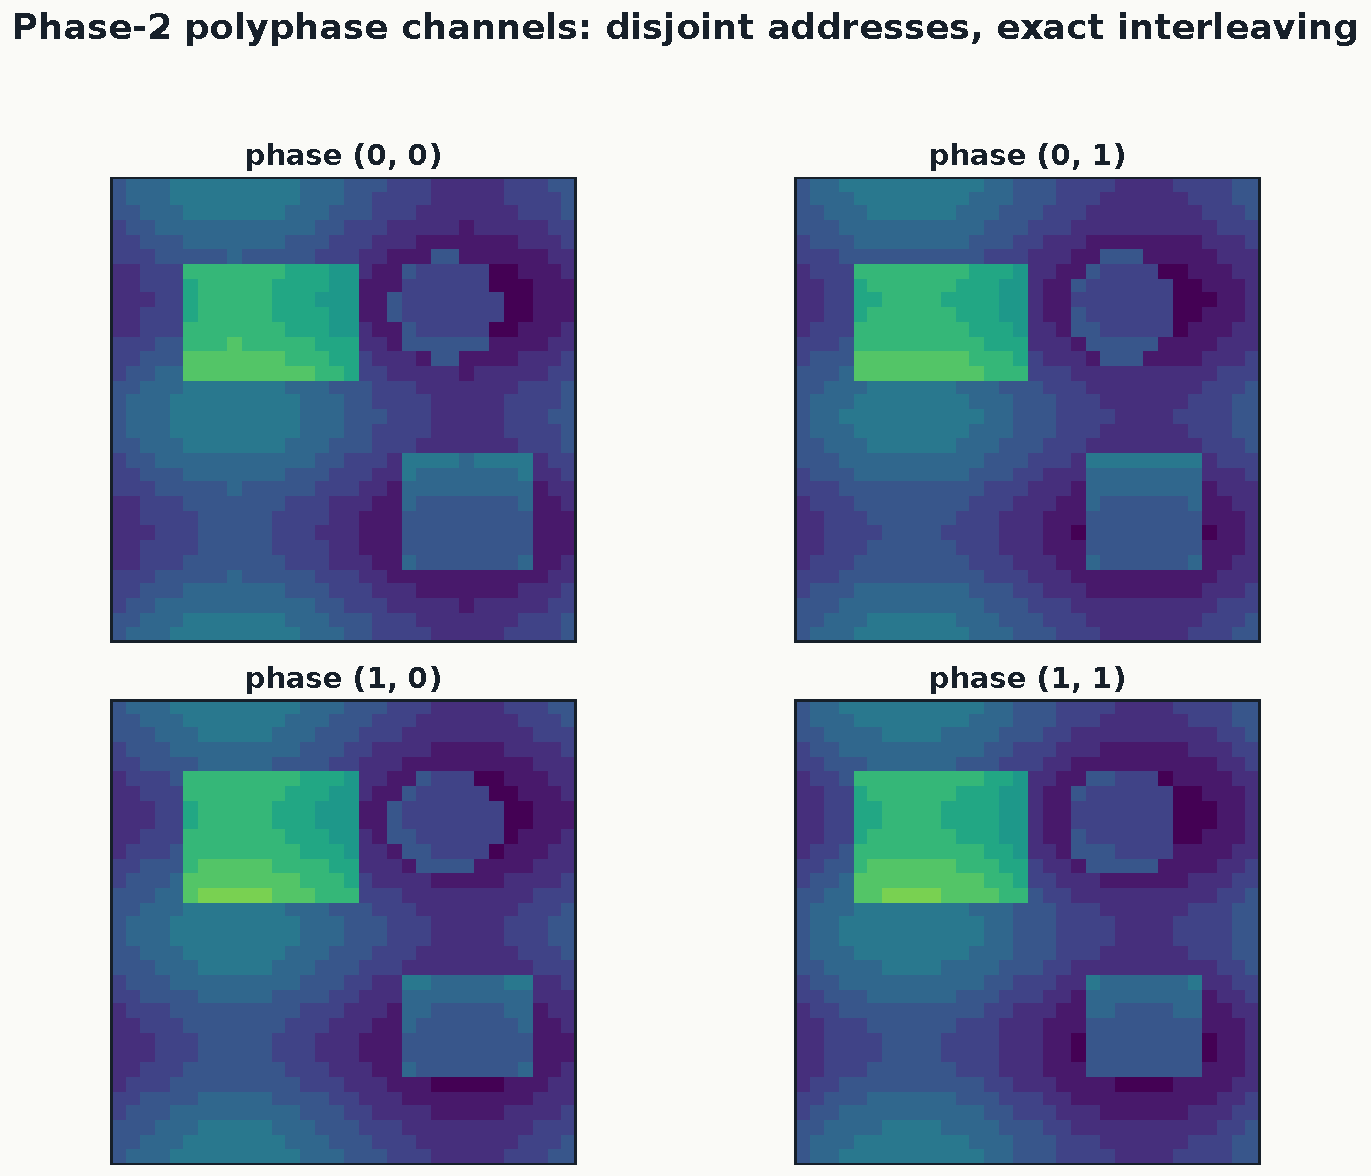
\includegraphics[width=.82\linewidth]{07_polyphase_channels.pdf}
\caption{Polyphase coordinates expose address classes without dropping samples.}
\end{figure}

\subsection{Categorical color packets}

A finite-valued frame can be encoded by the one-hot coordinates
\[
C_j[m,n]=\mathbf 1_{x[m,n]=j}.
\]
The original frame is recovered by the unique active color at each address.  This reconstruction is categorical rather than linear over the original scalar encoding, so it is kept as a separately typed exact atlas.

\begin{figure}[H]
\centering
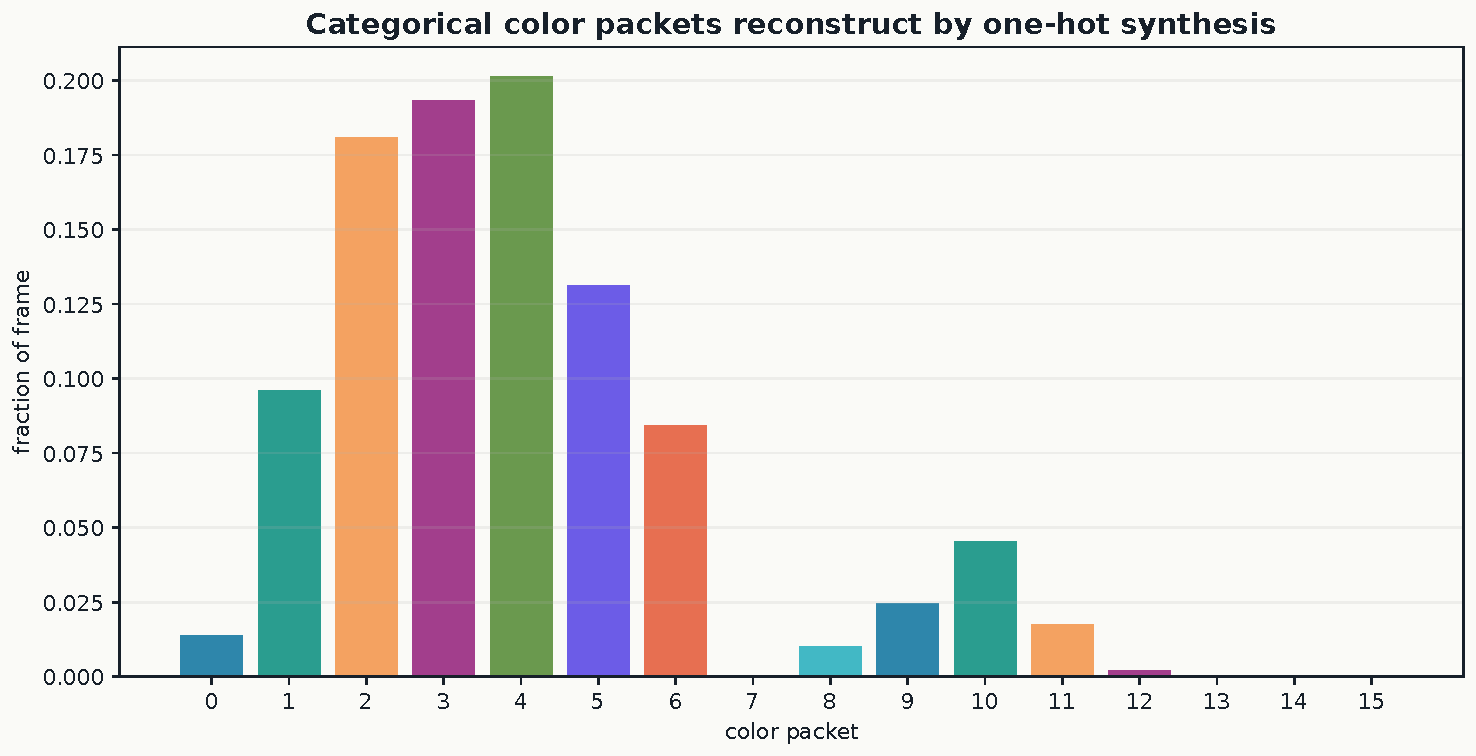
\includegraphics[width=.82\linewidth]{08_color_packets.pdf}
\caption{Color packets preserve categorical mass and exact label reconstruction.}
\end{figure}

\subsection{Reconstruction certificates}

\begin{certificate}[Exact atlas residuals]
Across the tested frames, the maximum observed residuals were
\[
\begin{array}{lr}
\toprule
\text{atlas}&\text{maximum absolute residual}\\
\midrule
\text{spatial}&0\\
\text{Fourier}&3.55\times10^{-15}\\
\text{Haar}&2.49\times10^{-14}\\
\text{polyphase-2}&0\\
\text{polyphase-4}&0\\
\text{categorical color}&0\\
\text{weighted multi-atlas frame}&5.33\times10^{-15}\\
\bottomrule
\end{array}
\]
The nonzero values are double-precision roundoff.
\end{certificate}

\begin{figure}[H]
\centering
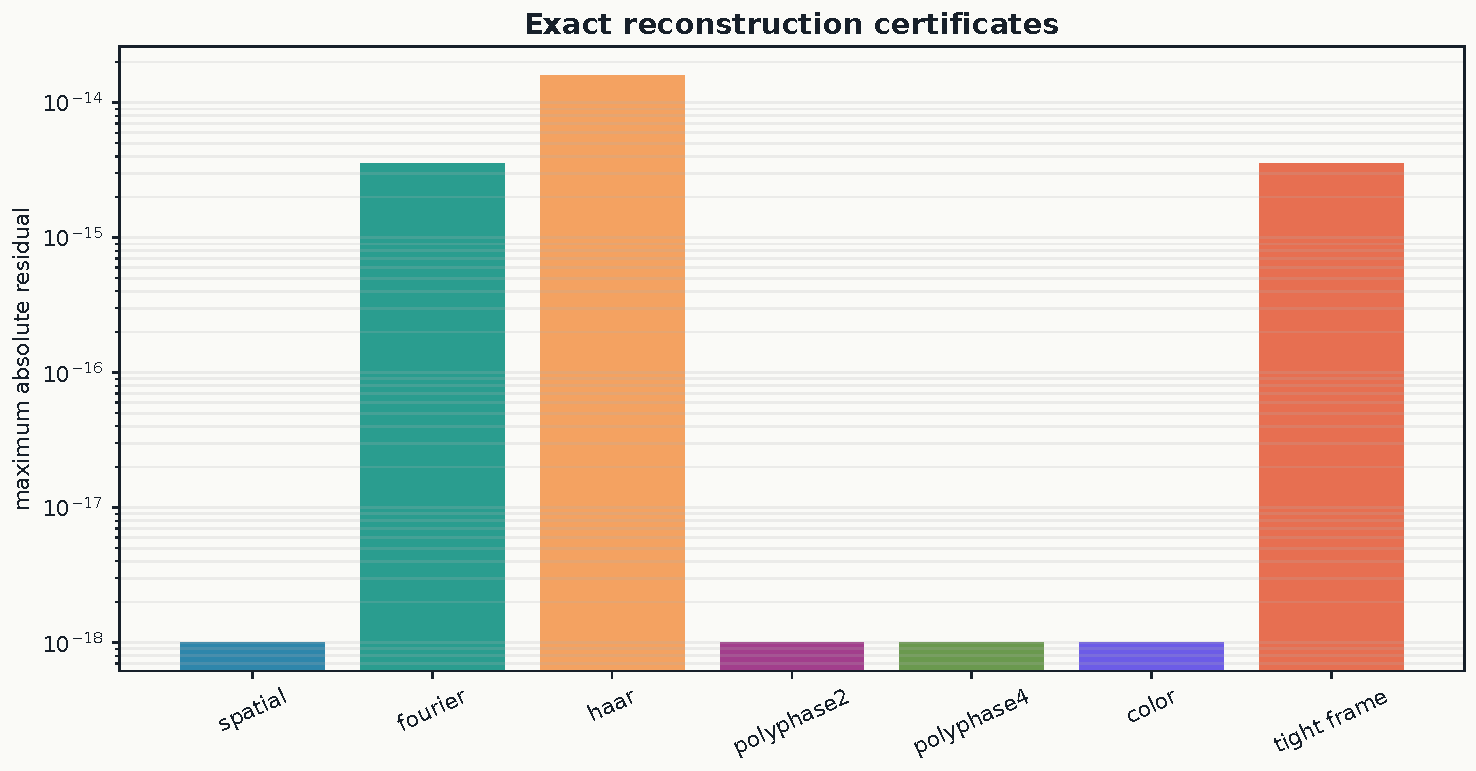
\includegraphics[width=.88\linewidth]{09_reconstruction_certificates.pdf}
\caption{The exact coordinate archive is accompanied by explicit numerical residuals.}
\end{figure}

\section{From exact coordinates to nested statistical states}

The exact archive is too large to place directly inside every candidate regression.  PR-LASM therefore computes interpretable summaries:
\begin{itemize}
\item pooled spatial values at several block sizes;
\item color masses and first spatial moments;
\item radial and angular Fourier energies plus low-frequency complex coefficients;
\item wavelet subband energies and coarse signed coefficients;
\item phase-channel means, deviations, and occupancy values;
\item connected-component, boundary, and change descriptors inherited from the interactive packetizer.
\end{itemize}

\begin{figure}[H]
\centering
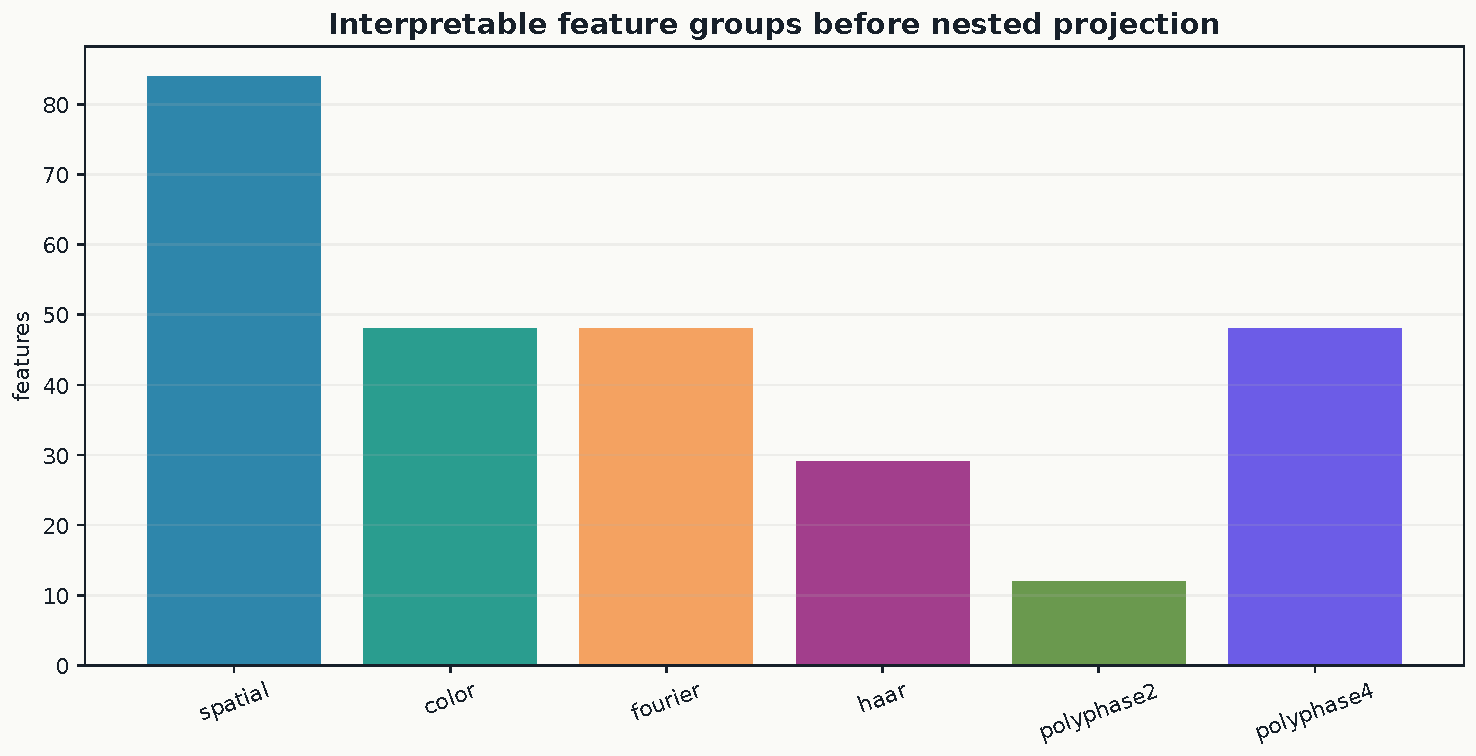
\includegraphics[width=.88\linewidth]{10_feature_portfolio.pdf}
\caption{The feature groups remain named before they are projected.}
\end{figure}

Let $r(x)\in\R^d$ be the concatenated feature vector.  A deterministic seeded QR factorization produces an orthonormal row system $Q$.  The nested states are
\[
z^{\mathrm{macro}}=Q_{1:k_1}r(x),
\qquad
z^{\mathrm{meso}}=Q_{1:k_2}r(x),
\qquad
z^{\mathrm{micro}}=Q_{1:k_3}r(x),
\]
with
\[
k_1<k_2<k_3<d.
\]
The supplied dimensions are $48$, $96$, and $192$.

\begin{boundary}[Projection status]
The nested states are deterministic compressions.  They are not claimed to reconstruct the original frame.  Exact reconstruction belongs to the coordinate archive, not to the statistical projections.
\end{boundary}

\section{Adaptive exact packet refinement}

A packet description should become finer only where the added structure improves the declared objective.  The release uses a complete Haar packet tree on a finite vector.

\begin{definition}[Complete pruning]
A set $\Lambda$ of packet-tree nodes is a complete pruning when every root-to-leaf path meets $\Lambda$ exactly once.
\end{definition}

\begin{theorem}[Exact mixed-depth synthesis]
Every complete pruning reconstructs the root signal exactly.
\end{theorem}

\begin{proof}
Every selected node either is the root or has a unique sibling selected or reconstructed at the same depth.  Applying inverse Haar synthesis to sibling pairs moves the selected representation one level upward.  Repeating finitely many times produces the root.  The complete-pruning condition prevents both missing branches and overlapping ancestor-descendant selections.
\end{proof}

Let $c(v)$ be any finite additive node cost.  Define recursively
\[
V(v)=
\min\left\{c(v),\sum_{u\in\operatorname{ch}(v)}V(u)\right\}.
\]

\begin{theorem}[Finite best-basis dynamic program]
The recursion returns a globally minimum-cost complete pruning in time linear in the number of tree nodes.
\end{theorem}

\begin{proof}
At a leaf, the only complete pruning is the leaf.  At an internal node, every complete pruning either keeps the node or uses complete prunings of both children.  Induction on depth proves optimality, and each node is evaluated once.
\end{proof}

\begin{figure}[H]
\centering
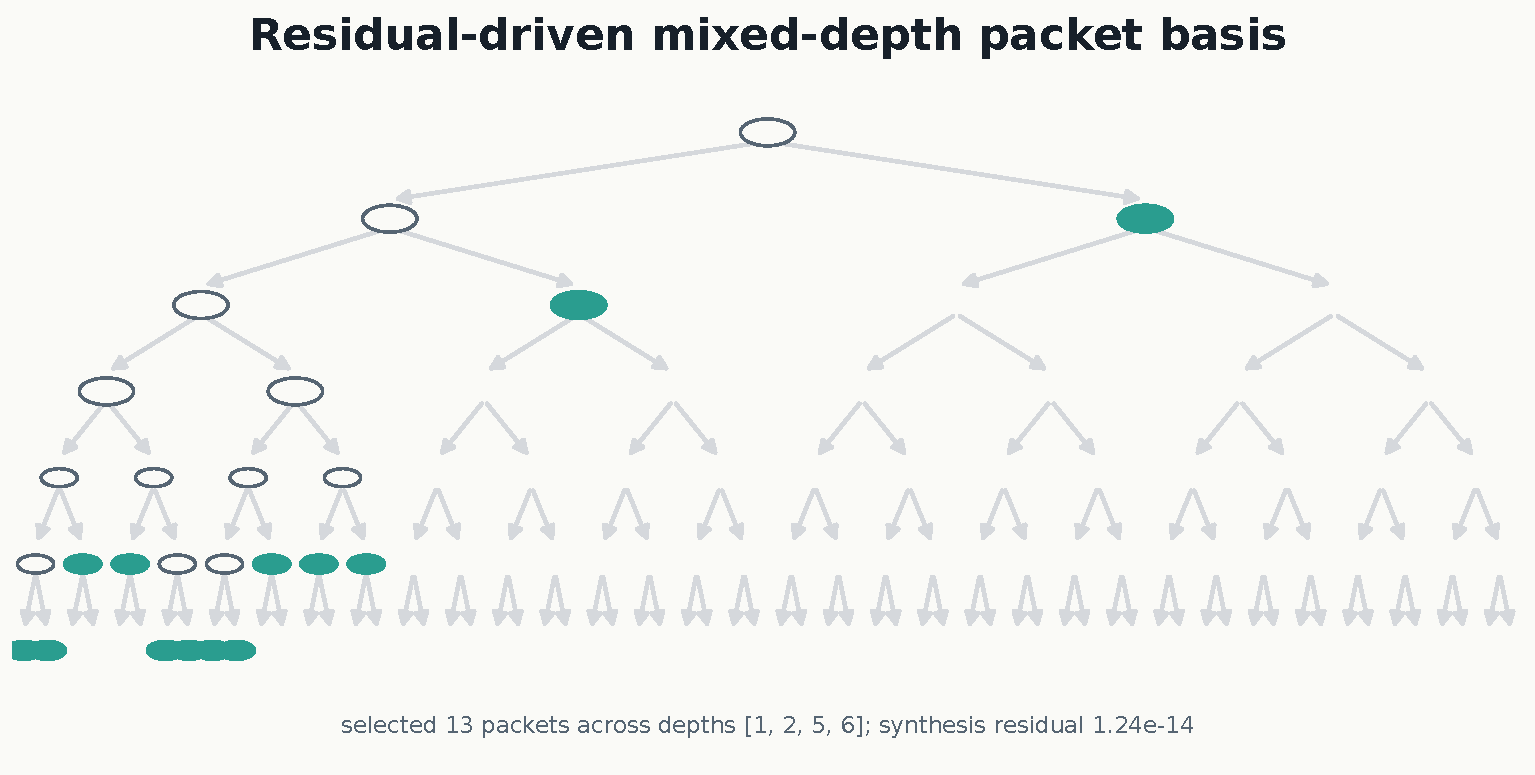
\includegraphics[width=.98\linewidth]{11_adaptive_packet_tree.pdf}
\caption{A mixed-depth complete pruning selected by dynamic programming.}
\end{figure}

\begin{figure}[H]
\centering
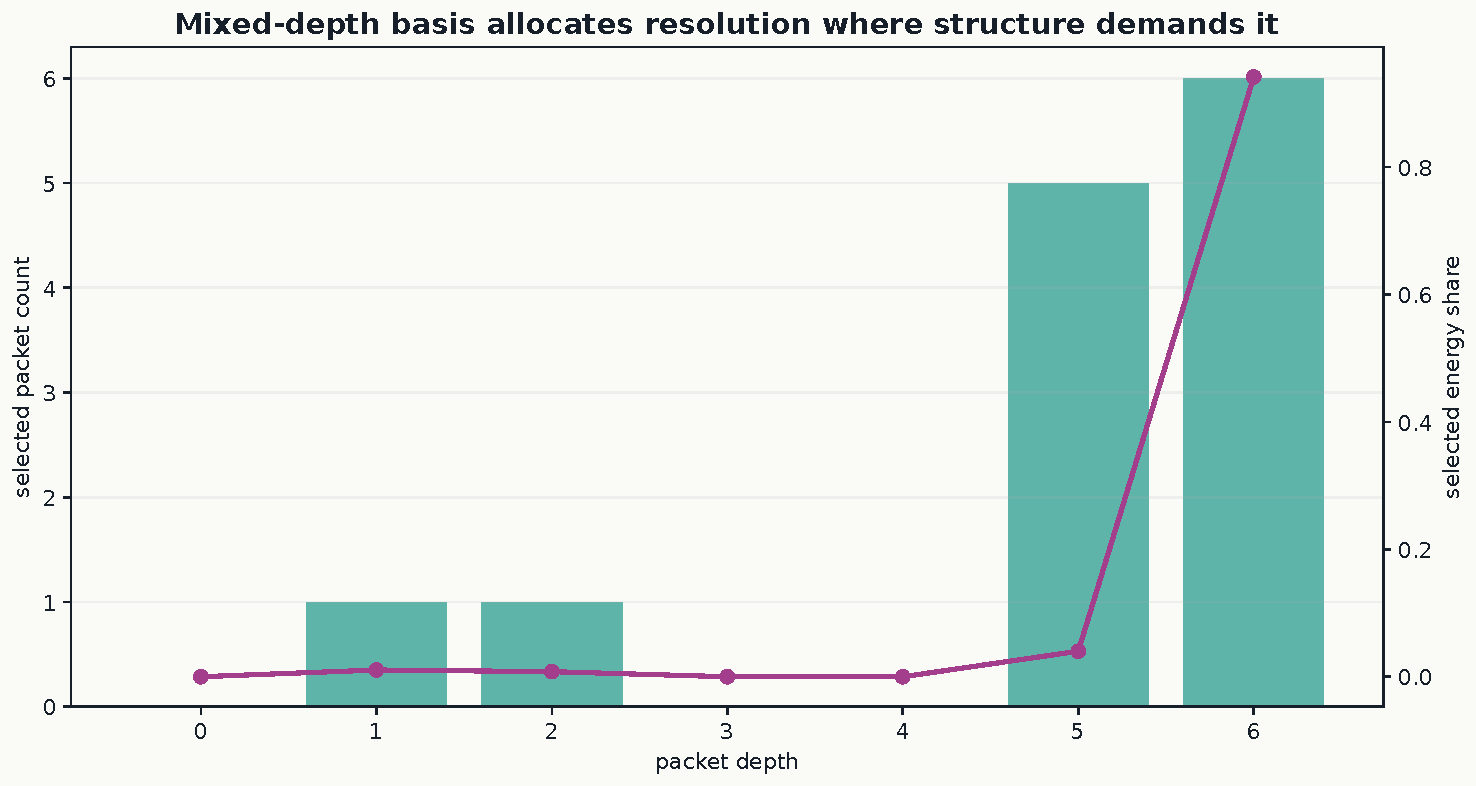
\includegraphics[width=.88\linewidth]{12_packet_basis_depths.pdf}
\caption{Selected packet counts and energy distribution across refinement depth.}
\end{figure}

In twenty-four structured frame tests, the selected basis used between $11$ and $61$ packets, with mean $32.58$.  The maximum reconstruction residual was $1.95\times10^{-14}$.

\section{The typed operator-program grammar}

A large signal model should not hide all mechanism uncertainty inside one dense matrix.  PR-LASM uses a typed program
\[
g=(a,r,f,\kappa),
\]
where $a$ is an atlas, $r$ is a resolution, $f$ is an operator family, and $\kappa$ contains family-specific ranks or periods.

For a packet state $z_t$, atlas features $q_t$, action features $u_t$, and memory state $m_t$, every program defines a design map
\[
\phi_g(z_t,q_t,u_t,m_t,t)\in\R^{d_g}.
\]
The target is
\[
y_t^{(g)}=
\begin{bmatrix}
 z_{t+1}^{(g)}-z_t^{(g)}\\
 R_t/100\\
 \Delta L_t\\
 \mathbf 1_{\mathrm{win}}\\
 \mathbf 1_{\mathrm{loss}}\\
 \mathbf 1_{\mathrm{changed}}
\end{bmatrix}.
\]

\begin{figure}[H]
\centering
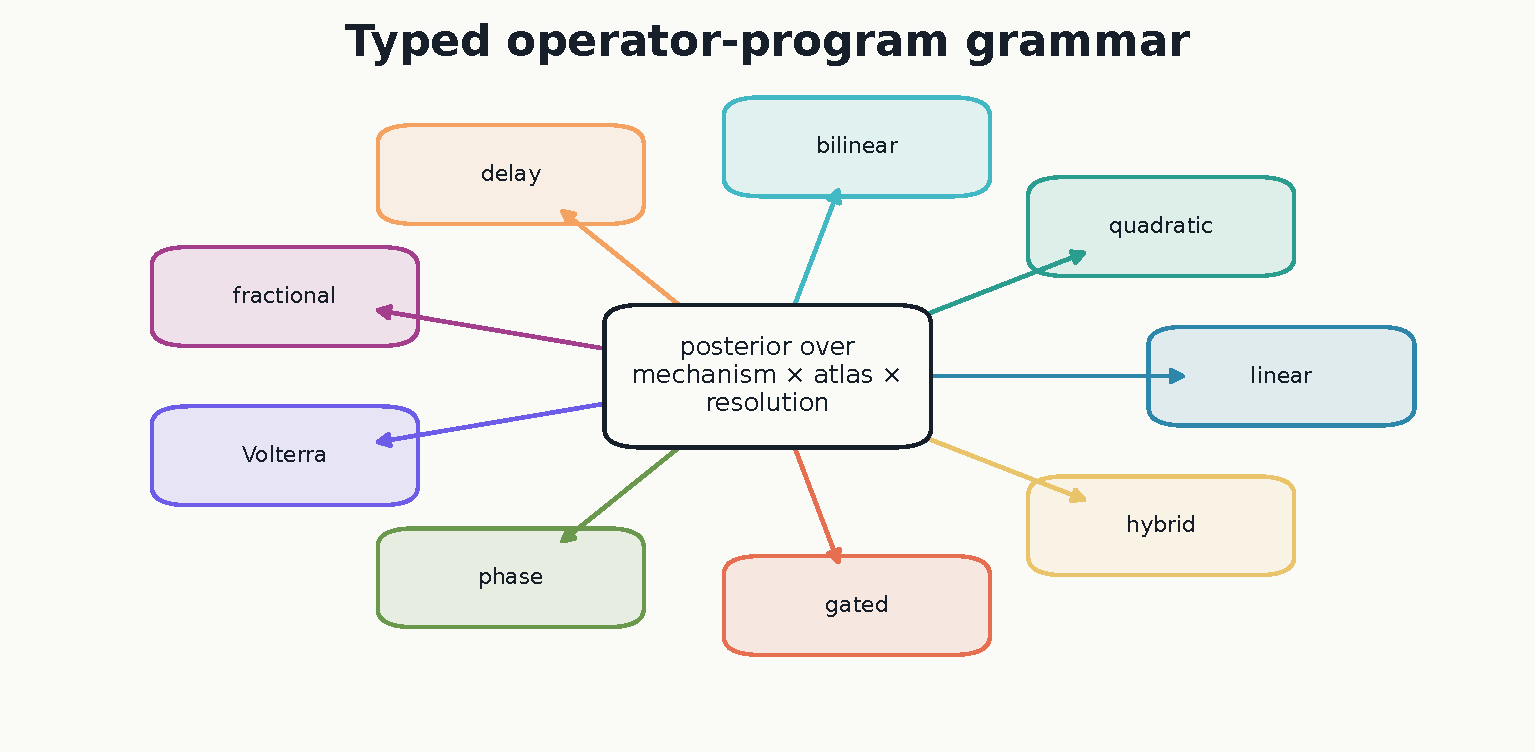
\includegraphics[width=.98\linewidth]{13_operator_grammar.pdf}
\caption{The finite grammar keeps mechanism names and penalties explicit.}
\end{figure}

\subsection{Linear and action-bilinear programs}

The basic linear program uses
\[
\phi_{\mathrm{lin}}=[1,z_t,q_t,u_t].
\]
The action-bilinear extension adds products
\[
z_{t,i}u_{t,j},
\qquad
q_{t,i}u_{t,j},
\]
for a declared low interaction rank.

\subsection{Quadratic packet interactions}

The quadratic program adds
\[
z_{t,i}z_{t,j},
\qquad
q_{t,i}q_{t,j},
\qquad i\le j,
\]
within a controlled rank.  This is a finite packet jet, not an unrestricted polynomial expansion.

\subsection{Delay and memory programs}

The delayed program appends $z_{t-1}$.  The power-memory packet is
\[
m_t^{\mathrm{pow}}
=
\frac{\displaystyle\sum_{\ell=1}^{H}\ell^{-\alpha}z_{t-\ell}}
{\displaystyle\sum_{\ell=1}^{H}\ell^{-\alpha}},
\]
while the exponential packet is
\[
m_t^{\mathrm{exp}}
=
\frac{\displaystyle\sum_{\ell=1}^{H}\rho^{\ell-1}z_{t-\ell}}
{\displaystyle\sum_{\ell=1}^{H}\rho^{\ell-1}}.
\]
The supplied defaults are $\alpha=0.68$ and $\rho=0.82$.

\begin{figure}[H]
\centering
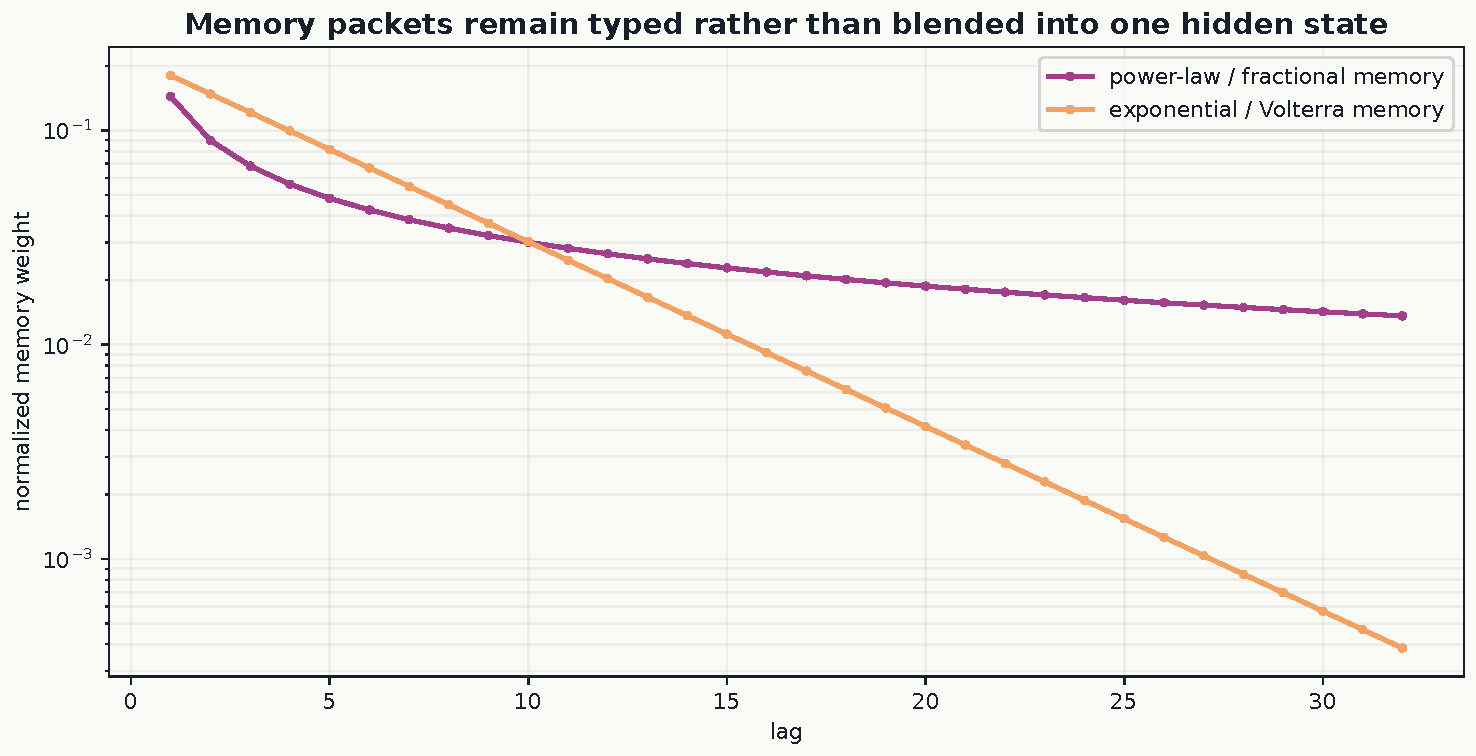
\includegraphics[width=.88\linewidth]{18_memory_kernels.pdf}
\caption{Power-law and exponential histories are retained as distinct memory mechanisms.}
\end{figure}

\subsection{Phase-conditioned programs}

For modulus $N$, the phase program appends the one-hot phase
\[
e_{t\bmod N}
\]
and interactions $z_{t,i}e_{t\bmod N}$.  Alternating, cyclic, or clocked dynamics therefore become linear in an expanded polyphase state.

\begin{figure}[H]
\centering
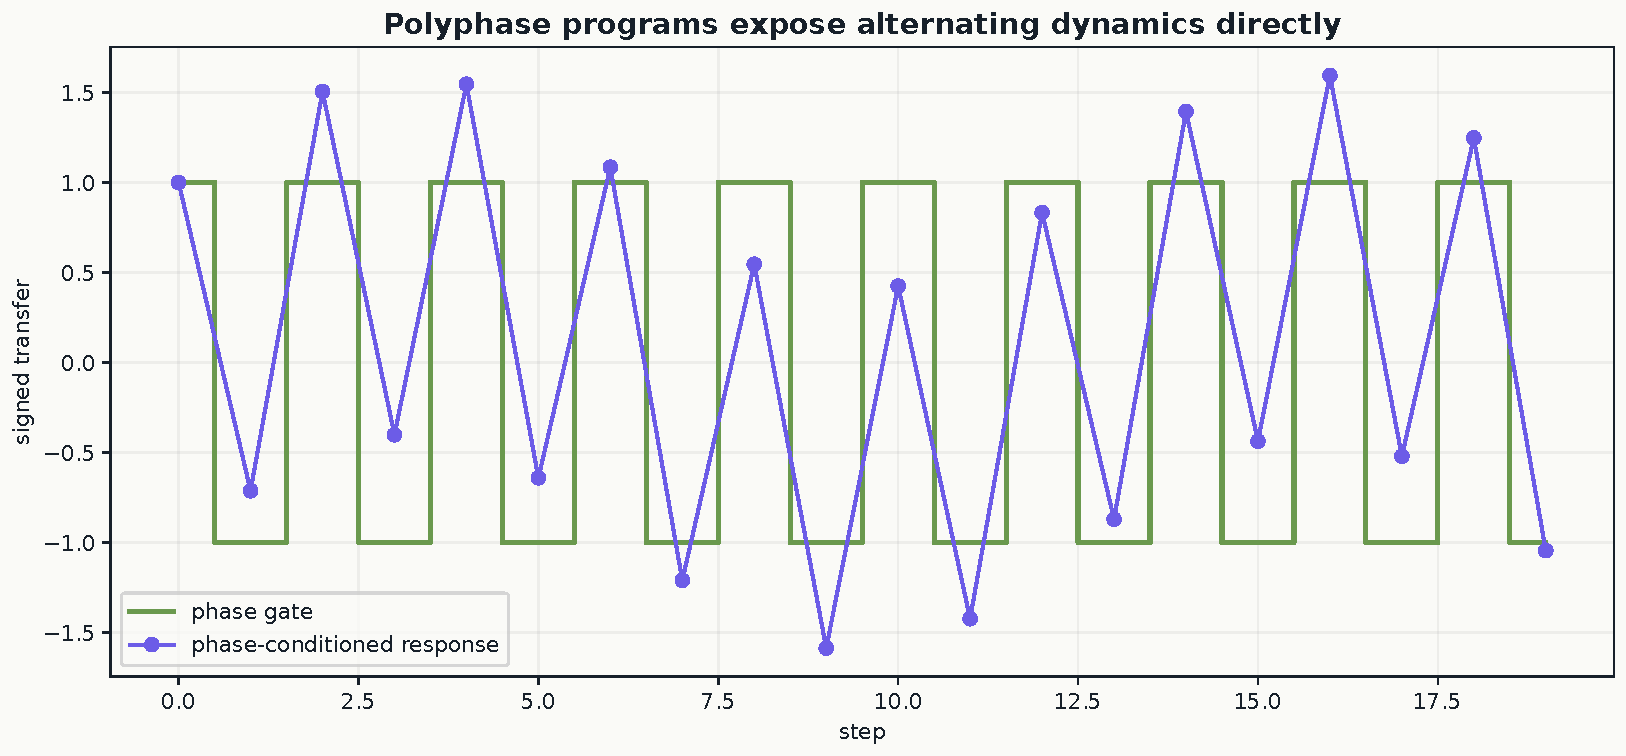
\includegraphics[width=.90\linewidth]{19_phase_conditioned_dynamics.pdf}
\caption{A periodic mechanism is simpler in its natural phase chart.}
\end{figure}

\subsection{Gated and hybrid programs}

The gated program uses a smooth gate
\[
\gamma_t=\frac{1}{1+e^{-4\bar q_t}}
\]
and appends $\gamma_tz_t$ and $(1-\gamma_t)z_t$.  The hybrid program contains a controlled combination of quadratic, delayed, power-memory, exponential-memory, and interaction terms.  Its higher prior penalty prevents it from winning merely because it has more columns.

\section{Bayesian operator selection}

For one program $g$, write
\[
Y=X_gB_g^\top+\varepsilon,
\]
with independent output variances and a normal-inverse-gamma prior.  If the prior precision is $\Lambda_0=\lambda_0I$, then
\[
\Lambda_n=\Lambda_0+X_g^\top X_g,
\qquad
M_n=Y^\top X_g\Lambda_n^{-1}.
\]
The posterior coefficient covariance is $\Lambda_n^{-1}$, and each output variance has an inverse-gamma posterior.

The implementation computes held-out Student predictive likelihood when enough rows are available.  The program log weight is
\[
\boxed{
W_g=
\ell_{\mathrm{pred}}(g)
-\lambda\,\operatorname{Complexity}(g)
-\eta\,\operatorname{Mechanisms}(g)
-\rho\,\operatorname{ResolutionPenalty}(g).}
\]
The posterior is
\[
p(g\mid D)=\frac{e^{W_g}}{\sum_he^{W_h}}.
\]

\subsection{Posterior predictive mixture}

If program $g$ predicts scalar vector $\mu_g$ with variance $V_g$, then
\[
\bar\mu=\sum_gp_g\mu_g,
\]
and the total predictive variance is
\[
\boxed{
V_{\mathrm{total}}
=
\underbrace{\sum_gp_gV_g}_{\text{within-program}}
+
\underbrace{\sum_gp_g(\mu_g-\bar\mu)^2}_{\text{between-program}}.}
\]
The second term is model disagreement and drives information-seeking behavior.

\section{Exact transition memory}

Each resolved frame receives a deterministic hash of its complete normalized array.  An observed public action defines a graph edge
\[
(s,a)\longmapsto s'.
\]
Repeated observations accumulate reward, progress, win, loss, and visit counts.

\begin{definition}[Deterministic replay edge]
An edge is deterministic when repeated replay of the same action history and current action returns the same state signature.  If two targets are observed, the edge is marked nondeterministic and is excluded from exact shortest-path reasoning.
\end{definition}

The graph supports:
\begin{itemize}
\item known winning and progressing actions;
\item untried actions at the current state;
\item frontier states with incomplete action coverage;
\item shortest known paths to a frontier;
\item loop and failure counts.
\end{itemize}

\begin{figure}[H]
\centering
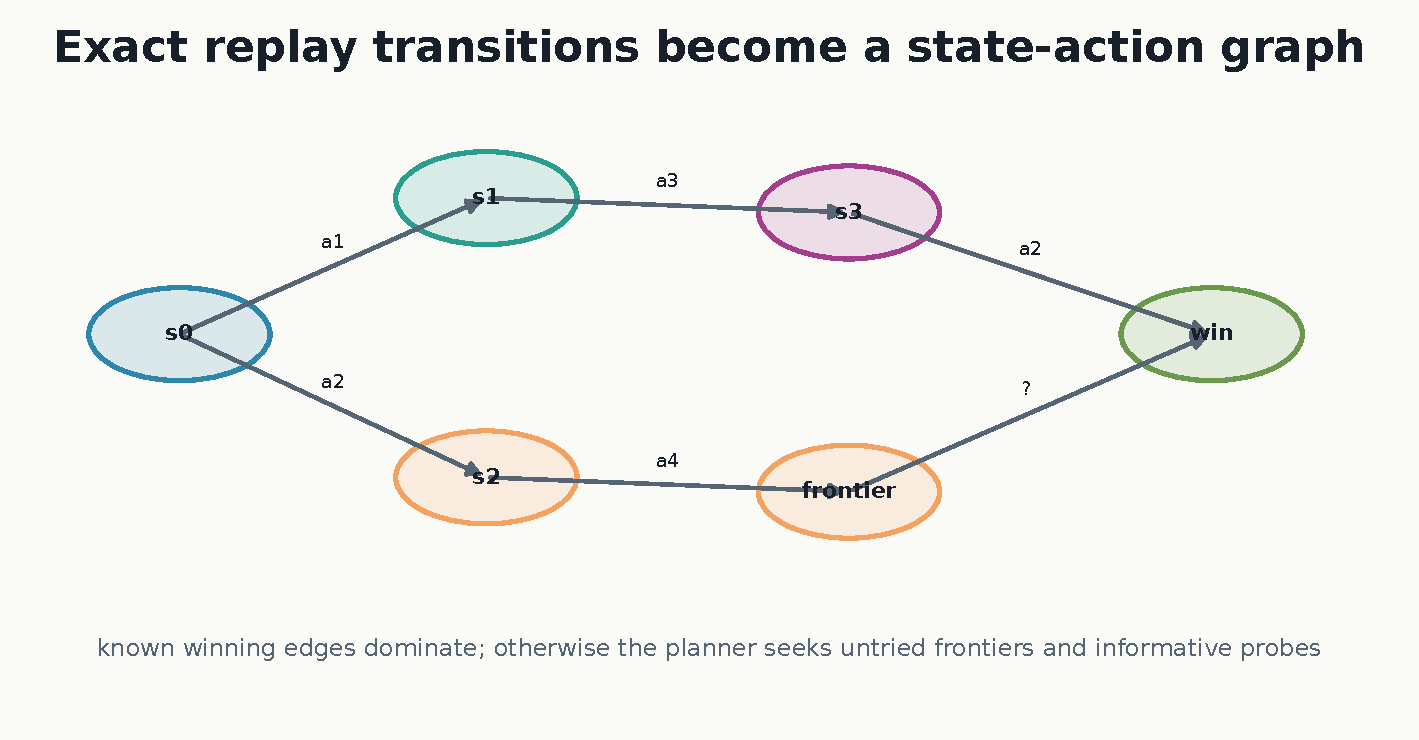
\includegraphics[width=.94\linewidth]{20_state_transition_graph.pdf}
\caption{Exact graph memory complements rather than replaces the learned world model.}
\end{figure}

\begin{proposition}[Replay safety rule]
If replay of the committed history produces a signature different from the expected current signature, all later replay probes are disabled for that run.
\end{proposition}

This rule sacrifices probe efficiency rather than treating a nondeterministic or hidden-state environment as deterministic.

\section{Active planning}

For candidate action $a$, the planner forms a utility
\[
\begin{aligned}
U(a)=&\ \widehat R(a)
+\lambda_L\widehat{\Delta L}(a)
+\lambda_W\widehat p_{\mathrm{win}}(a)
-\lambda_D\widehat p_{\mathrm{loss}}(a)\\
&+\lambda_N\operatorname{Novelty}(a)
+\lambda_I\operatorname{Information}(a)
-\lambda_V\operatorname{Variance}(a)\\
&+\lambda_H\operatorname{RoleHistory}(a)
-\lambda_Q\operatorname{RepeatCount}(a)^2
+\lambda_F\mathbf1_{\mathrm{untried}}.
\end{aligned}
\]
Exact probe outcomes replace the corresponding predicted terms.  Known graph wins and progress receive dominant bonuses.  This ordering ensures that an already observed winning action is not ignored because a statistical model has not yet fit it.

\begin{figure}[H]
\centering
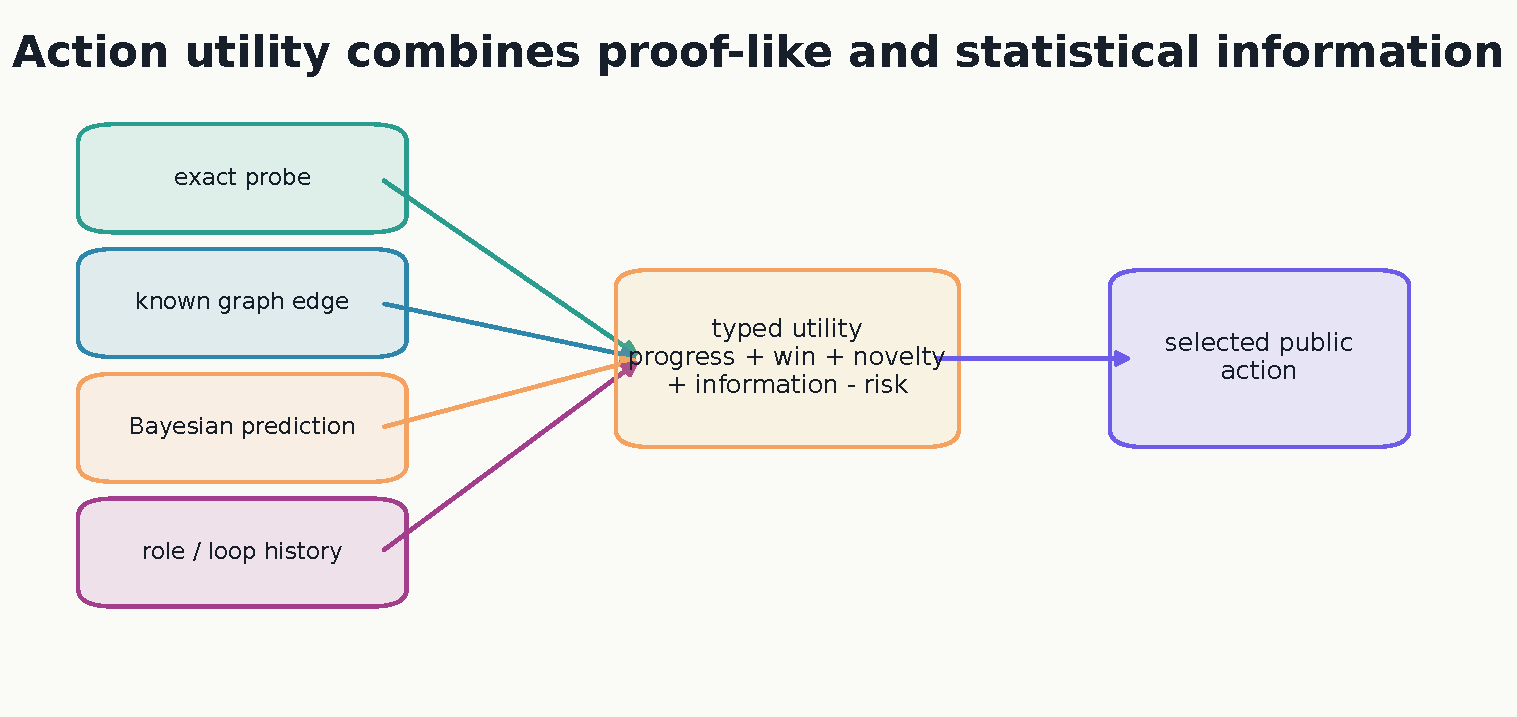
\includegraphics[width=.94\linewidth]{23_active_planning_utility.pdf}
\caption{The planner combines exact and probabilistic evidence without merging their logical types.}
\end{figure}

\section{Residual-driven model evolution}

The model loop is
\[
\boxed{
\text{analyze exactly}
\to
\text{fit typed posterior}
\to
\text{predict and act}
\to
\text{measure residual}
\to
\text{refine selectively}.}
\]
A residual can trigger:
\begin{itemize}
\item a finer statistical projection;
\item a different atlas expert;
\item a packet-tree split;
\item a delay or memory mechanism;
\item an action interaction;
\item an explicit graph edge rather than a learned approximation.
\end{itemize}

\begin{figure}[H]
\centering
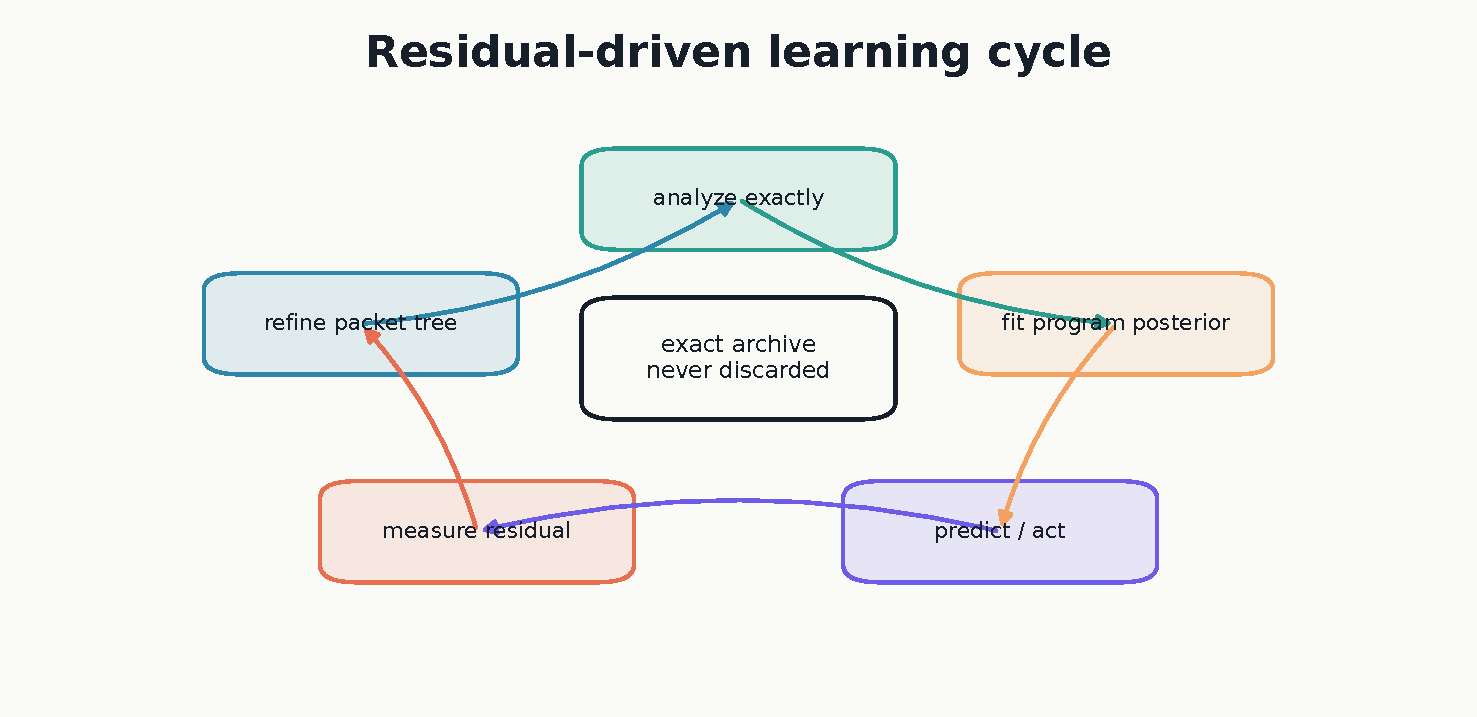
\includegraphics[width=.92\linewidth]{24_residual_refinement_cycle.pdf}
\caption{The exact archive remains fixed while the predictive view changes.}
\end{figure}

\section{Algorithms}

\subsection{Exact multi-atlas packetization}

\begin{lstlisting}[language=Python,caption={Core exact analysis contract.}]
analysis = analyzer.analyze(frame)
assert max(analysis.reconstruction_residuals().values()) < tolerance
exact = analysis.tight_frame_synthesis(weights)
assert max_abs(exact - frame) < tolerance
features = analyzer.feature_groups(analysis)
z_macro = Q[:48] @ concatenate(features)
z_meso  = Q[:96] @ concatenate(features)
z_micro = Q[:192] @ concatenate(features)
\end{lstlisting}

\subsection{Program fitting}

\begin{lstlisting}[language=Python,caption={Typed Bayesian program comparison.}]
for program in grammar:
    X = stack(program.design_transition(row) for row in records)
    Y = stack(program.targets(row) for row in records)
    posterior = normal_inverse_gamma_fit(X_train, Y_train)
    score = predictive_log_likelihood(posterior, X_valid, Y_valid)
    weight[program] = score - complexity_penalty(program)
probability = softmax(weight)
\end{lstlisting}

\clearpage
\subsection{Active agent loop}

\begin{lstlisting}[language=Python,caption={PR-LASM planning loop.}]
while budget_remains and not terminal:
    packets = exact_and_statistical_analysis(observation)
    candidates = public_action_candidates(observation, packets)
    probes = deterministic_replay_probes(history, candidates)
    if enough_records:
        world_model.fit(memory)
    scores = utility(candidates, probes, graph, posterior, memory)
    action = argmax(scores)
    next_observation = environment.step(action)
    record_transition(observation, action, next_observation)
    update_graph_and_residuals()
\end{lstlisting}

\section{Computational organization}

Structured transforms are applied before dense learning.  The exact Fourier transform uses FFT structure, the Haar transform uses local butterfly operations, and polyphase extraction is a permutation of addresses.  Dense linear algebra is confined to projected states and program-specific design matrices.

\begin{figure}[H]
\centering
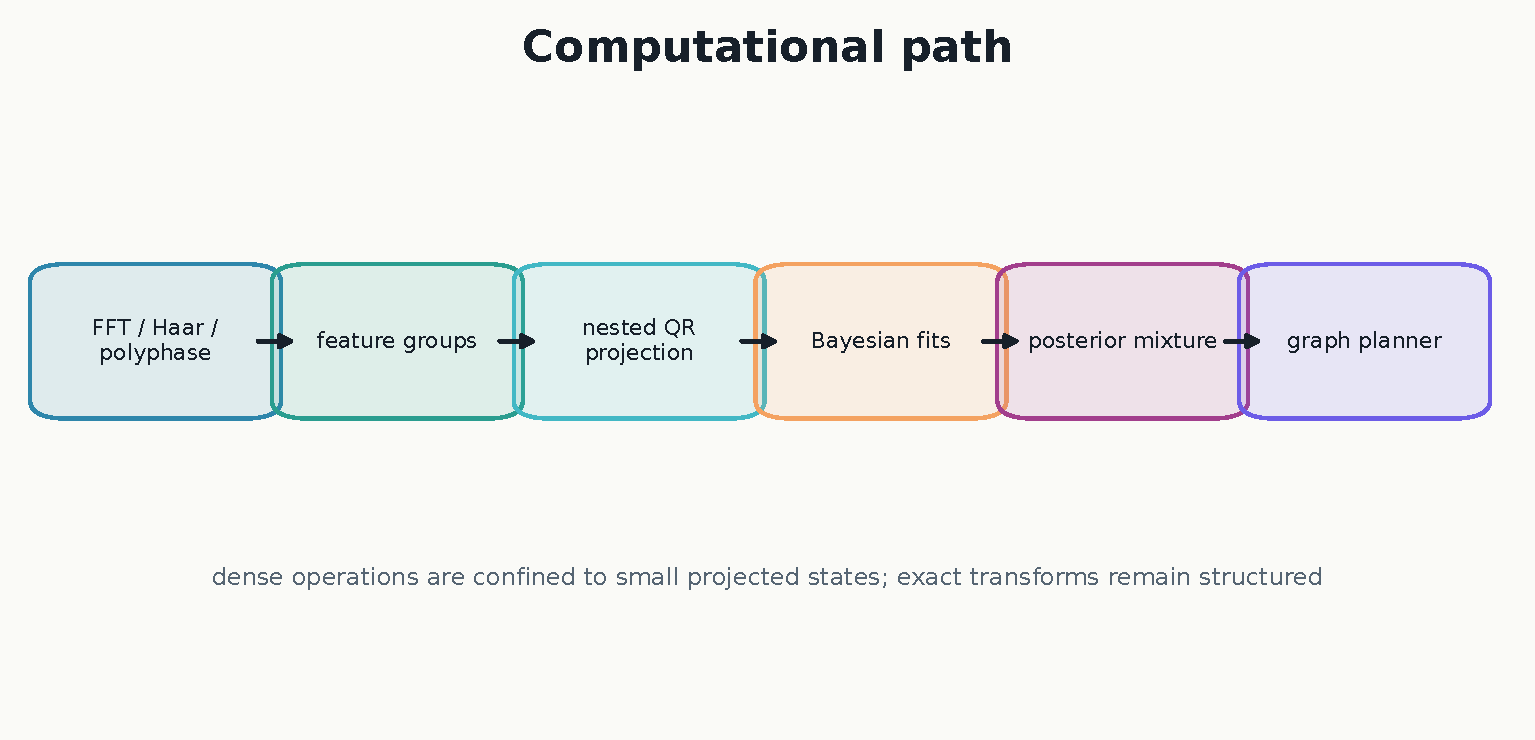
\includegraphics[width=.98\linewidth]{25_computational_path.pdf}
\caption{The implementation keeps full-resolution transforms structured and small-state inference dense.}
\end{figure}

For $n$ signal coordinates, $A$ exact unitary atlases, projected state dimension $k$, $G$ candidate programs, and $m$ observed transitions, the dominant modeled costs are:
\[
\begin{array}{ll}
\text{FFT atlas}&O(n\log n),\\
\text{Haar atlas}&O(n),\\
\text{polyphase atlas}&O(n),\\
\text{feature projection}&O(dk),\\
\text{one regression fit}&O(md_g^2+d_g^3),\\
\text{all program fits}&\displaystyle\sum_{g=1}^GO(md_g^2+d_g^3).
\end{array}
\]
The architecture is designed so that $d_g$ is controlled by the selected rank and resolution rather than by the full signal dimension.

\section{Controlled program-identification benchmark}

The mechanism benchmark is deliberately algebraic.  It does not claim to reproduce the uncertainty of arbitrary physical or interactive data.  Its purpose is narrower: verify that when data are generated by one typed mechanism, the implementation can distinguish that mechanism from simpler alternatives on held-out records.

Seven systems were generated:
\begin{enumerate}
\item Fourier-atlas linear transfer;
\item spatial quadratic interaction;
\item delayed portfolio dynamics;
\item Fourier power-memory dynamics;
\item portfolio exponential-memory dynamics;
\item phase-two polyphase dynamics;
\item color-gated dynamics.
\end{enumerate}

For each system, $84$ records were used for fitting and $36$ independent records for testing.  The target-driving variables absent from simpler candidate programs were independently randomized.  This prevents the benchmark from being solved by time-index memorization.

\begin{certificate}[Mechanism and atlas identification]
The highest posterior family matched the declared generating family in all seven systems.  The highest posterior atlas matched the declared atlas in all seven systems.
\end{certificate}

\begin{figure}[H]
\centering
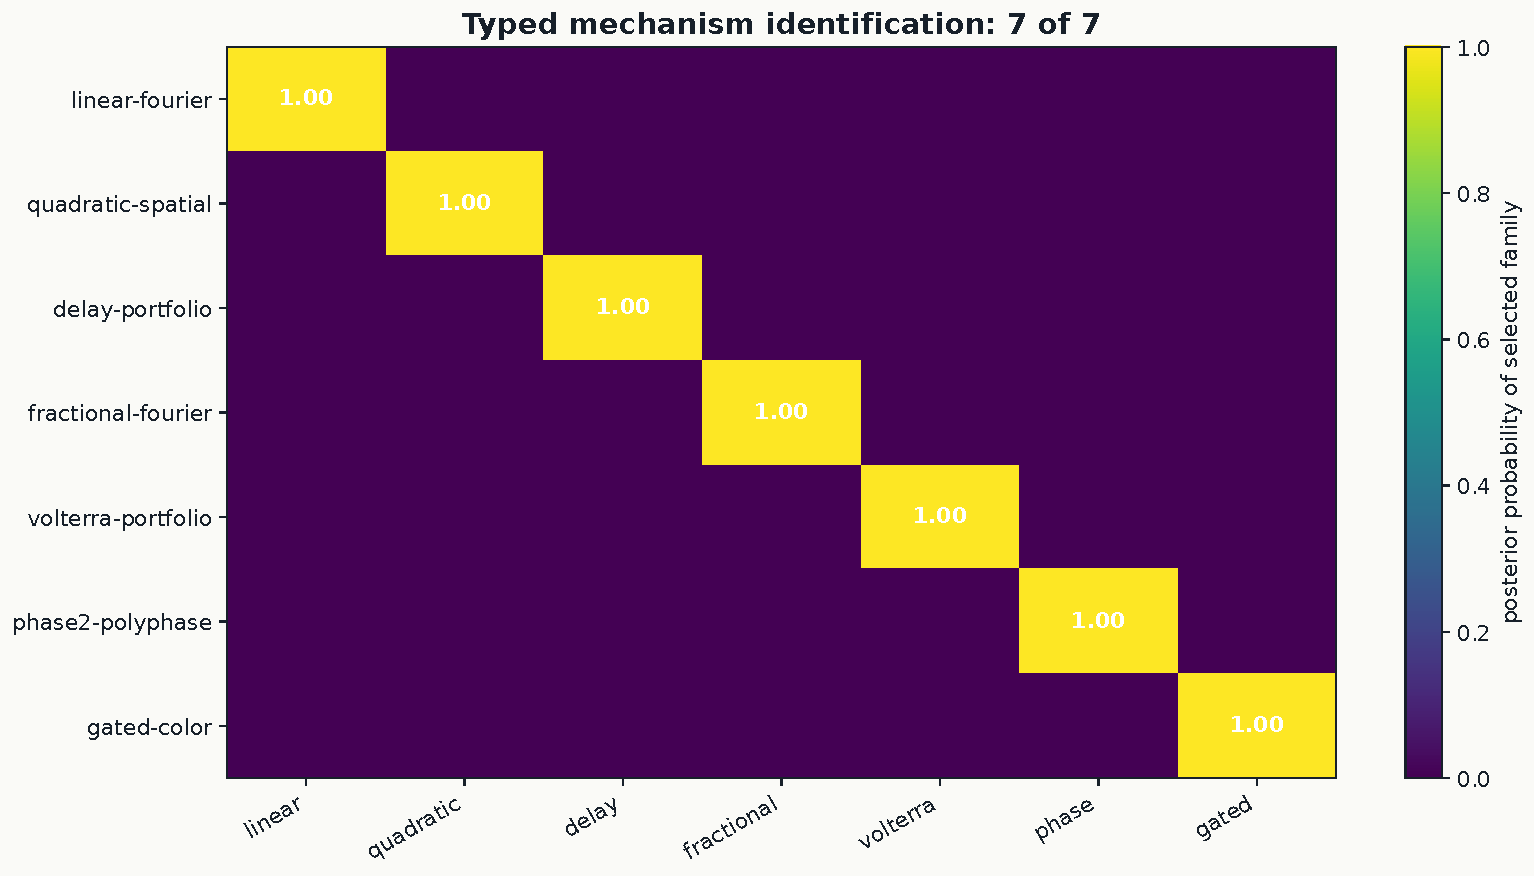
\includegraphics[width=.96\linewidth]{14_mechanism_identification.pdf}
\caption{Every controlled mechanism was identified by its typed posterior.}
\end{figure}

\begin{figure}[H]
\centering
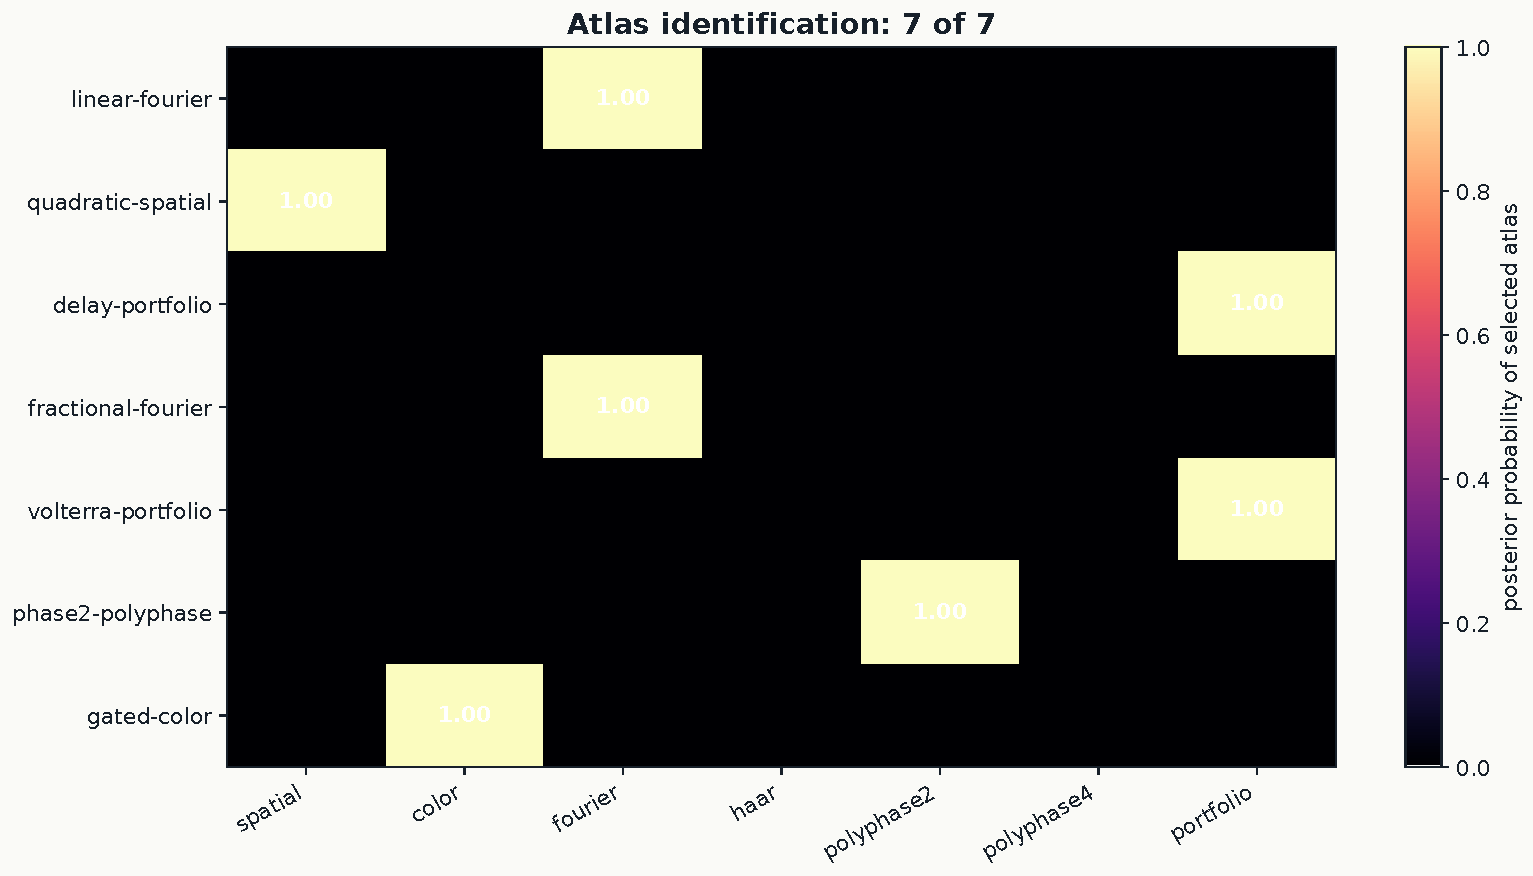
\includegraphics[width=.96\linewidth]{15_atlas_identification.pdf}
\caption{Every controlled coordinate atlas was identified.}
\end{figure}

\subsection{Linear ablation}

The baseline is one linear macro-resolution program using the portfolio atlas.  PR-LASM uses the full typed posterior.  The test-state RMSE values are:

\begin{table}[H]
\centering
\small
\begin{tabular}{lrrr}
\toprule
system&linear baseline&PR-LASM&ratio\\
\midrule
linear Fourier&0.2449&0.0221&0.0903\\
quadratic spatial&0.2708&0.1240&0.4580\\
delay portfolio&0.3112&0.0629&0.2020\\
fractional Fourier&0.2735&0.0654&0.2393\\
Volterra portfolio&0.2793&0.0642&0.2300\\
phase-two polyphase&0.1465&0.0436&0.2978\\
gated color&0.0502&0.0385&0.7674\\
\bottomrule
\end{tabular}
\caption{Held-out state-prediction RMSE.  The benchmark is controlled and mechanism-specific.}
\end{table}

\begin{figure}[H]
\centering
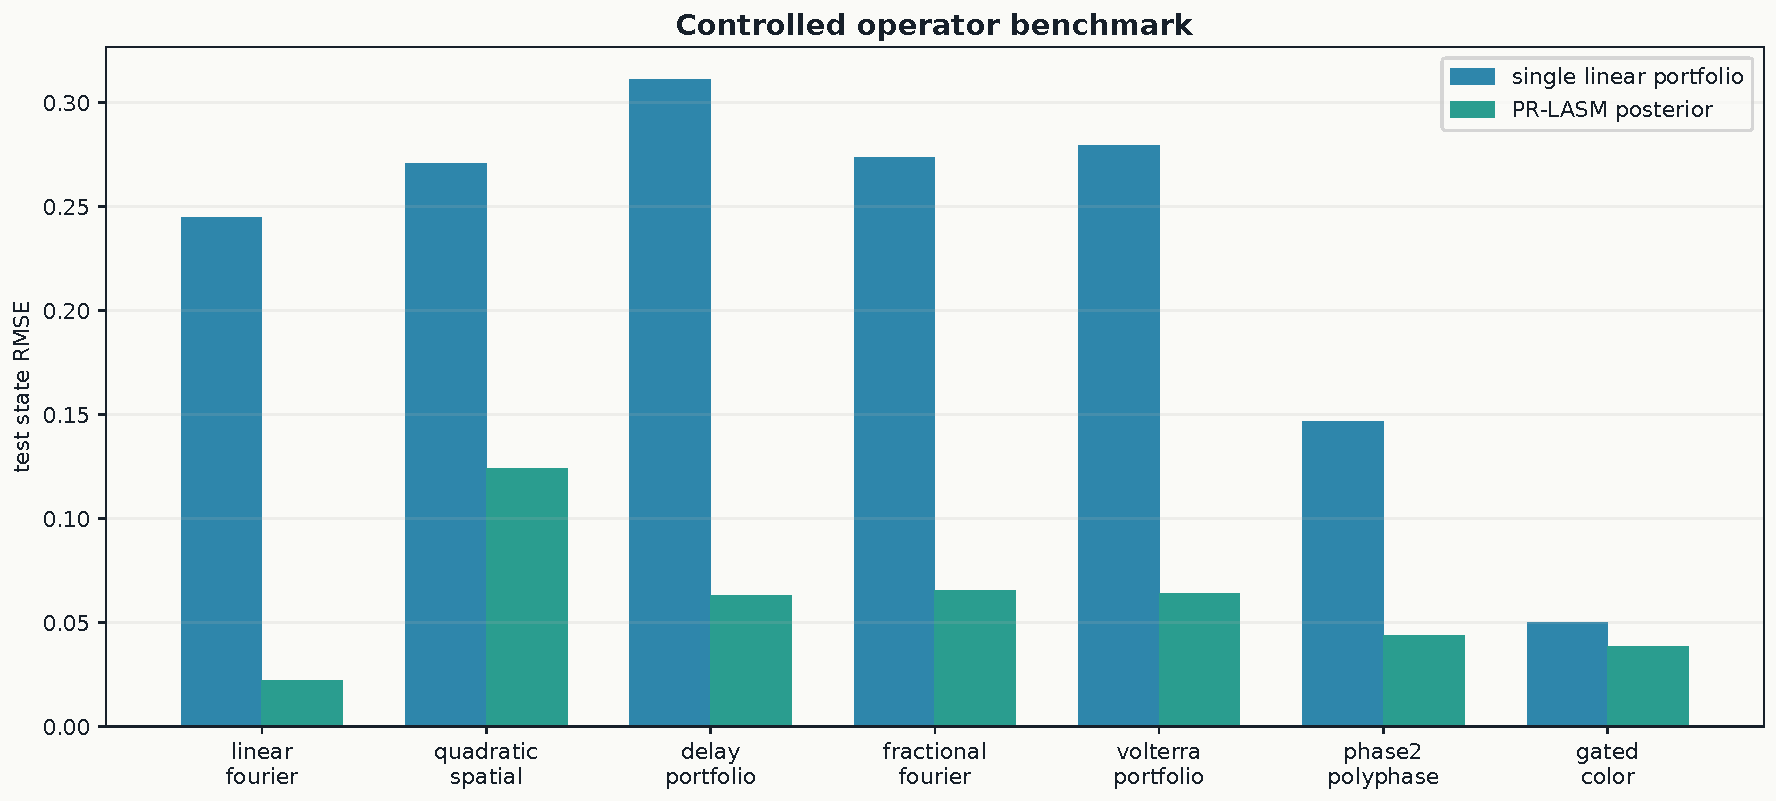
\includegraphics[width=.96\linewidth]{16_operator_rmse.pdf}
\caption{The full typed model versus the single linear portfolio baseline.}
\end{figure}

\begin{figure}[H]
\centering
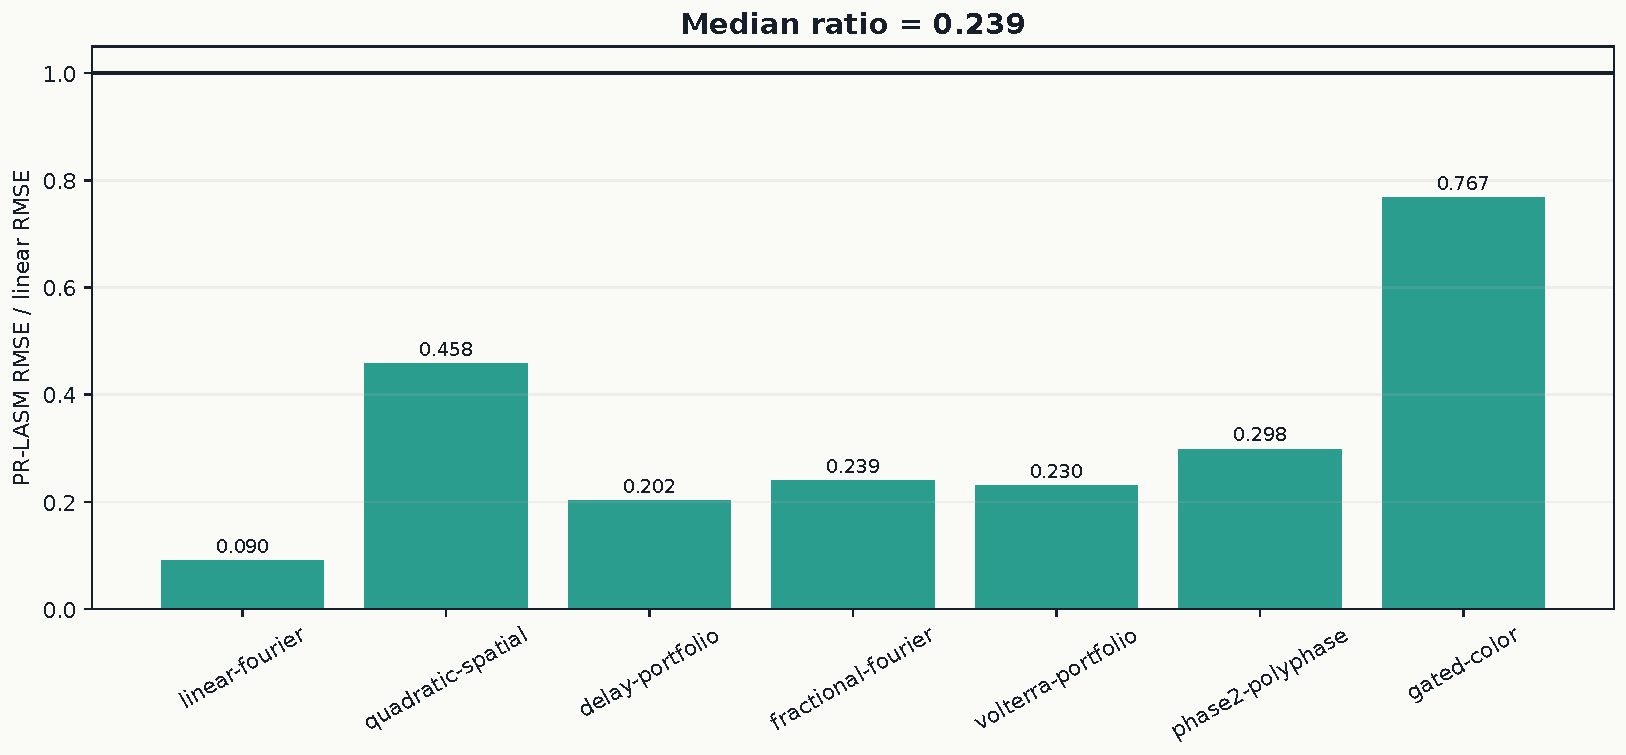
\includegraphics[width=.92\linewidth]{17_rmse_ratios.pdf}
\caption{All seven state RMSE ratios are below one; the median is $0.2393$.}
\end{figure}

\begin{boundary}[Interpretation of the controlled benchmark]
The result verifies program construction, posterior comparison, and held-out prediction when the generating family belongs to the supplied grammar.  It does not prove that the grammar contains the mechanism of an arbitrary environment.
\end{boundary}

\section{Deterministic interactive benchmarks}

Four source-blind environments test the integrated planning loop:
\begin{itemize}
\item a five-step action sequence;
\item a spatial click target;
\item a grid-navigation task with walls;
\item a six-step alternating phase switch.
\end{itemize}
All expose only observations and public actions.  Deterministic replay is available, so the graph and probe system can be tested exactly.

\begin{certificate}[Interactive systems]
PR-LASM solved all four systems.  The recorded committed-action counts were $38$, $1$, $29$, and $14$.  The corresponding graph sizes ranged from one to twenty states and from twelve to thirty-two transition edges.
\end{certificate}

\begin{figure}[H]
\centering
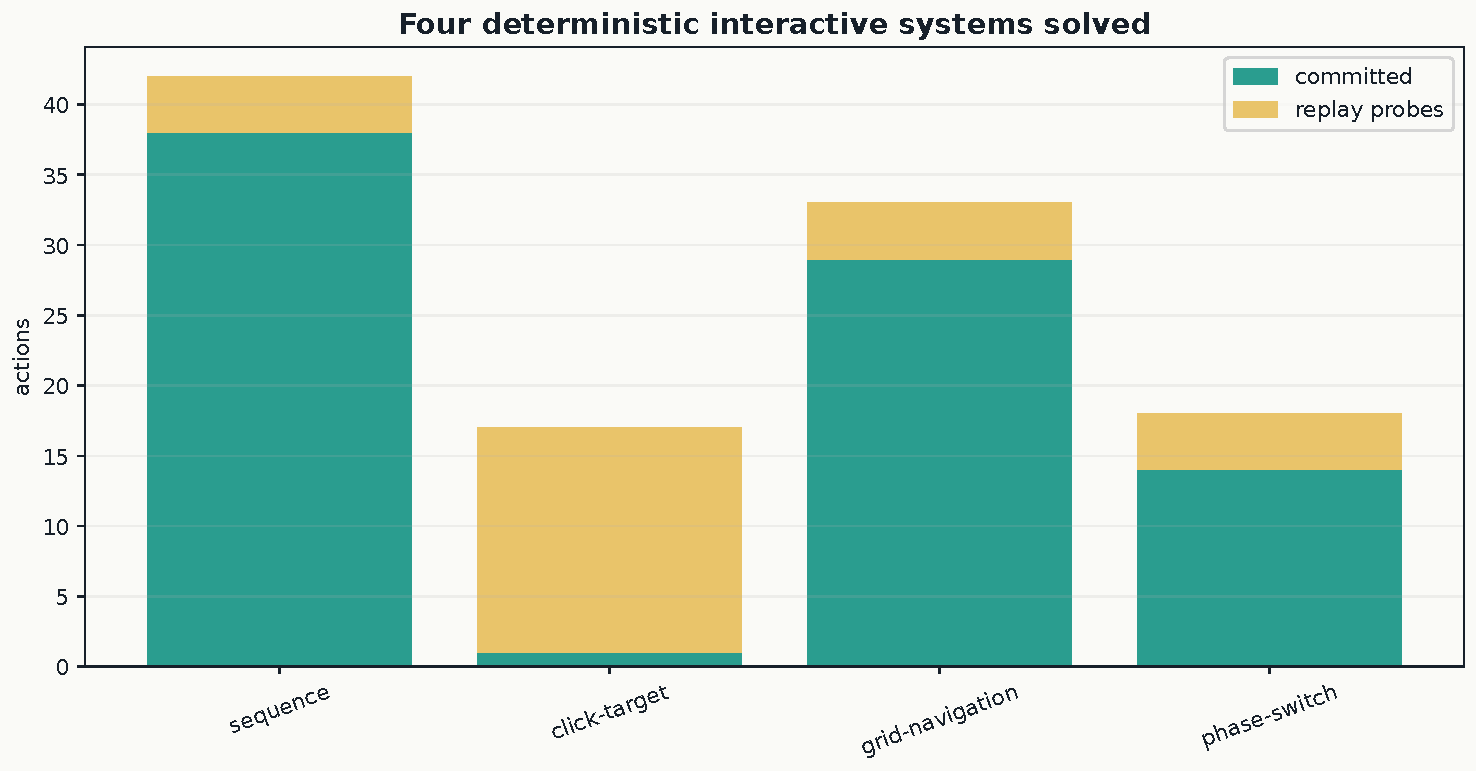
\includegraphics[width=.90\linewidth]{21_agent_actions.pdf}
\caption{Committed actions and replay probes in the four interactive systems.}
\end{figure}

\begin{figure}[H]
\centering
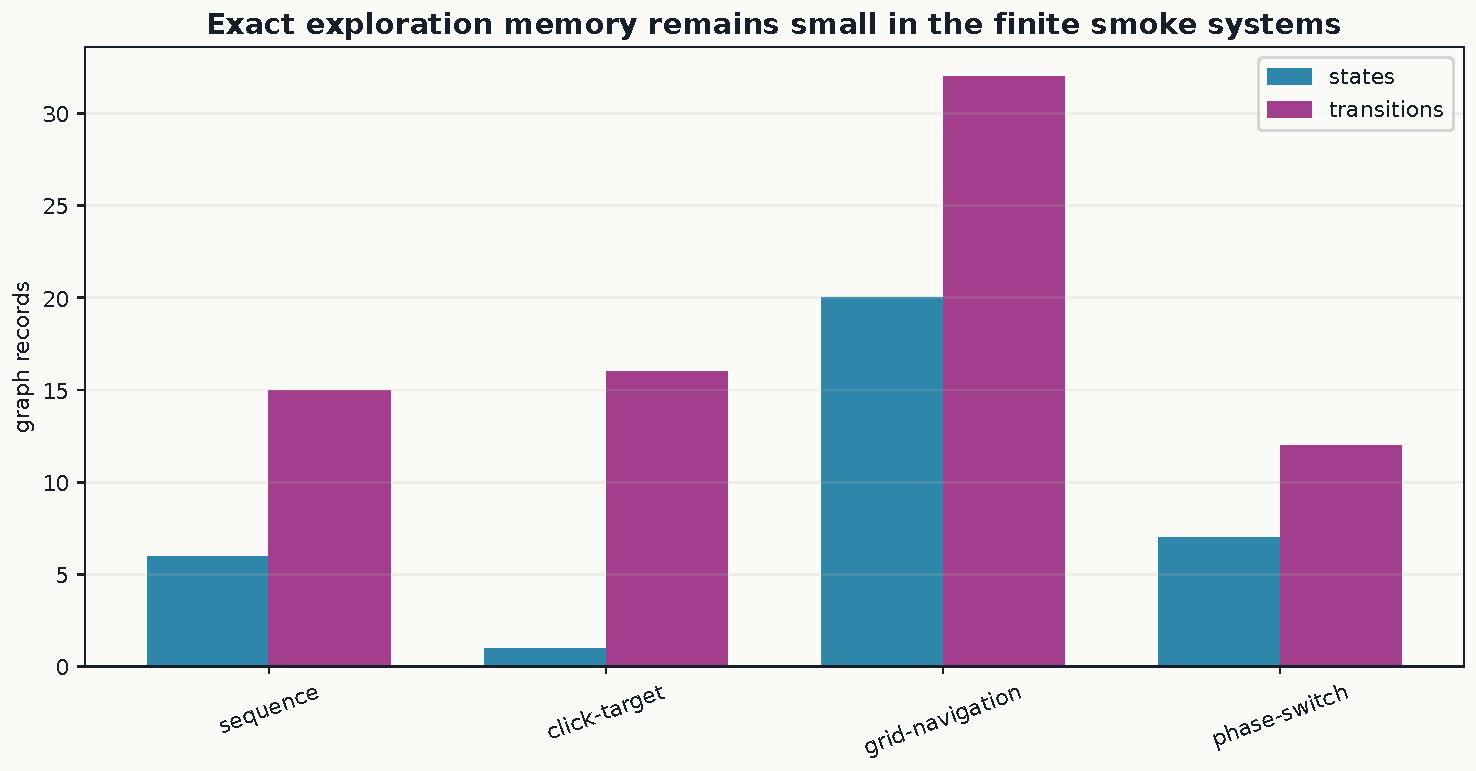
\includegraphics[width=.90\linewidth]{22_agent_graph_sizes.pdf}
\caption{Exact graph memory remained compact in the finite smoke tasks.}
\end{figure}

\section{The supplied twenty-five-environment suite}

The release bundles twenty-five local environment trees.  Static validation checks metadata, source presence, source syntax, the expected game-class structure, and prohibited network or process-control imports.  All twenty-five trees pass.

The supplied baseline-action totals vary substantially, so the runner retains per-environment budgets rather than using one small global cap.

\begin{figure}[H]
\centering
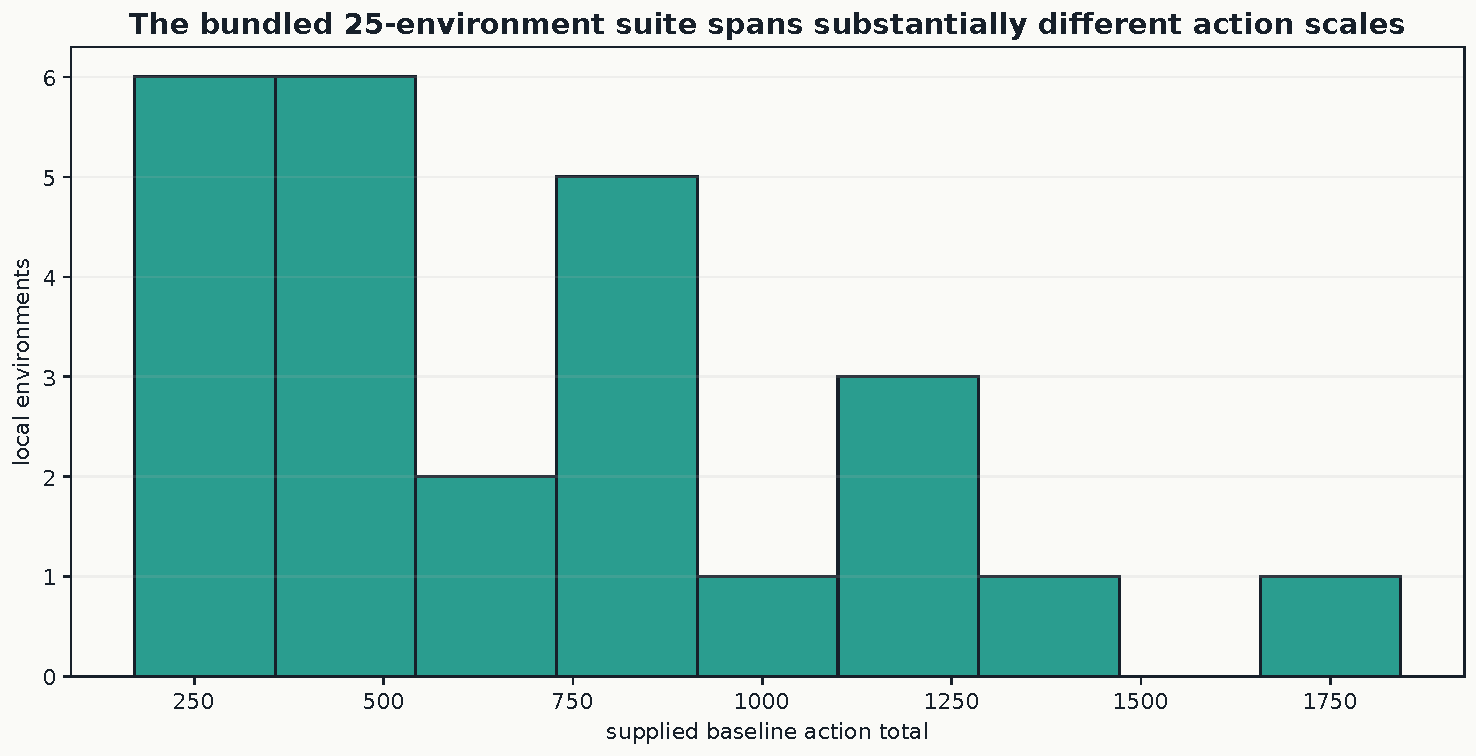
\includegraphics[width=.90\linewidth]{26_arc25_action_scale.pdf}
\caption{Distribution of supplied baseline-action totals across the local suite.}
\end{figure}

\begin{figure}[H]
\centering
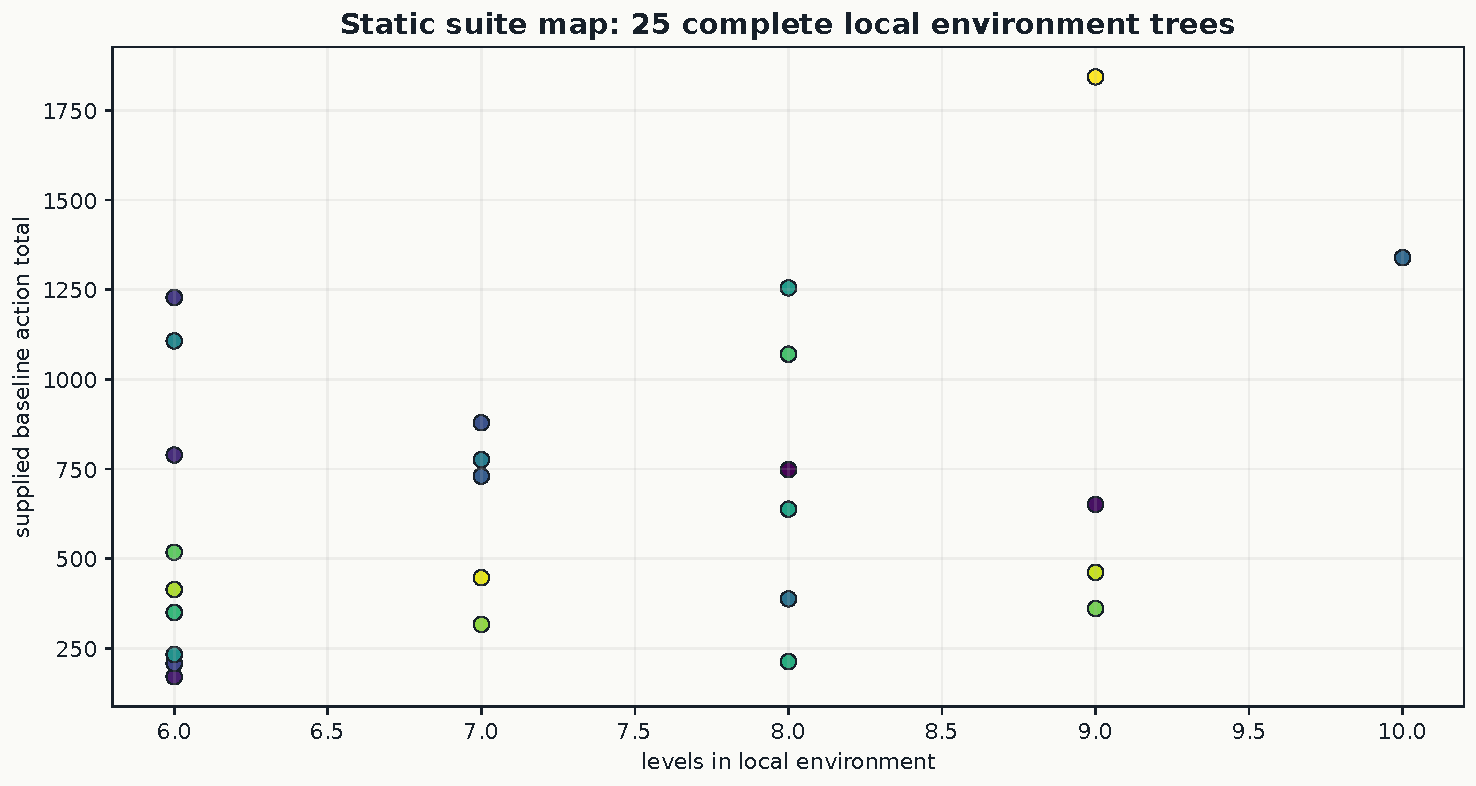
\includegraphics[width=.90\linewidth]{27_arc25_suite_map.pdf}
\caption{Level counts and baseline-action totals for the twenty-five local environment trees.}
\end{figure}

\begin{boundary}[No official execution claim]
The official local runtime was not available in the present build container.  Therefore this paper reports no solved count, score, or timing for the twenty-five environments.  The release includes offline run scripts for the target machine and preserves the original strict network guard.
\end{boundary}

\section{Software architecture}

\begin{longtable}{L{0.37\linewidth}L{0.55\linewidth}}
\toprule
module&role\\
\midrule
\endfirsthead
\toprule
module&role\\
\midrule
\endhead
\texttt{exact\_atlas.py}&unitary Fourier, orthonormal Haar, polyphase, categorical color, projector queries, tight-frame synthesis\\
\texttt{lasm\_packetizer.py}&exact archive, named feature groups, deterministic nested projections\\
\texttt{lasm\_refinement.py}&complete packet trees, mixed-depth synthesis, best-basis dynamic programming\\
\texttt{lasm\_programs.py}&typed design maps for linear, nonlinear, phase, delay, and memory mechanisms\\
\texttt{lasm\_model.py}&Bayesian fitting, posterior weights, uncertainty decomposition, action prediction\\
\texttt{lasm\_memory.py}&committed states, lag packets, power memory, exponential memory, role statistics\\
\texttt{lasm\_graph.py}&exact transition edges, nondeterminism marking, frontier and path queries\\
\texttt{lasm\_agent.py}&replay probes, utility scoring, graph updates, source-blind interactive loop\\
\texttt{lasm\_benchmark.py}&exactness, controlled operator, and interactive benchmarks\\
\texttt{lasm\_cli.py}&benchmark, smoke, single-environment, and suite commands\\
\bottomrule
\end{longtable}

The command
\begin{lstlisting}
python -m komorebi_arc3_offline.lasm_cli benchmark \
  --output results/pr_lasm_benchmark
\end{lstlisting}
regenerates the benchmark ledgers.  The PowerShell wrappers provide the same operation on Windows.

\section{Verification}

\begin{certificate}[Automated suite]
The complete source release passes
\[
\boxed{36/36\text{ automated tests}.}
\]
The tests include all seventeen inherited offline-runner tests and nineteen PR-LASM tests covering exact atlas reconstruction, Fourier packet completeness, polyphase synthesis, wavelet subband synthesis, tight-frame reconstruction, deterministic packetization, mixed-depth best-basis reconstruction, graph frontiers, seven typed program-identification cases, and four interactive systems.
\end{certificate}

\begin{figure}[H]
\centering
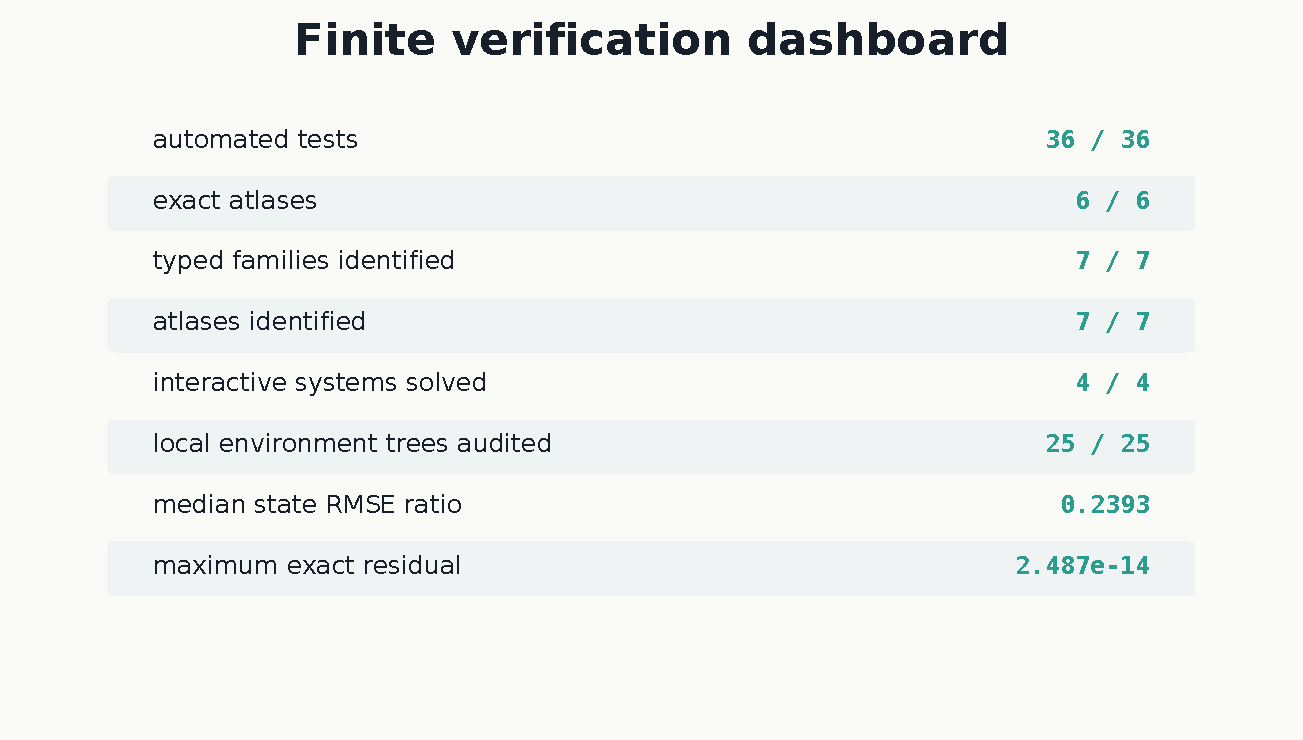
\includegraphics[width=.92\linewidth]{29_verification_dashboard.pdf}
\caption{Summary of the finite verification state.}
\end{figure}

\section{Claim ledger}

\begin{longtable}{L{0.36\linewidth}L{0.18\linewidth}L{0.37\linewidth}}
\toprule
statement&status&boundary\\
\midrule
\endfirsthead
\toprule
statement&status&boundary\\
\midrule
\endhead
Per-atlas packet reconstruction&theorem&finite unitary atlas and complete coordinate selectors\\
Weighted multi-atlas synthesis&theorem&finite family of unitary atlases with positive weights\\
Categorical color reconstruction&exact construction&finite one-hot palette\\
Mixed-depth packet pruning&theorem&finite complete binary packet tree\\
Best-basis dynamic program&theorem&finite additive node cost\\
Bayesian regression formulas&exact finite formulas&declared normal-inverse-gamma model\\
Typed program selection&finite certificate&seven controlled systems generated from the supplied grammar\\
RMSE improvement&finite certificate&controlled held-out benchmark only\\
State-action graph&exact finite data structure&deterministic edges only\\
Interactive solutions&finite certificate&four bundled deterministic systems\\
Twenty-five environment integrity&static certificate&source trees, not executed games\\
Official environment score&not claimed&official local runtime absent from build container\\
Universal operator discovery&not claimed&finite declared grammar\\
AGI&not claimed&outside the mathematical and empirical scope\\
\bottomrule
\end{longtable}

\begin{figure}[H]
\centering
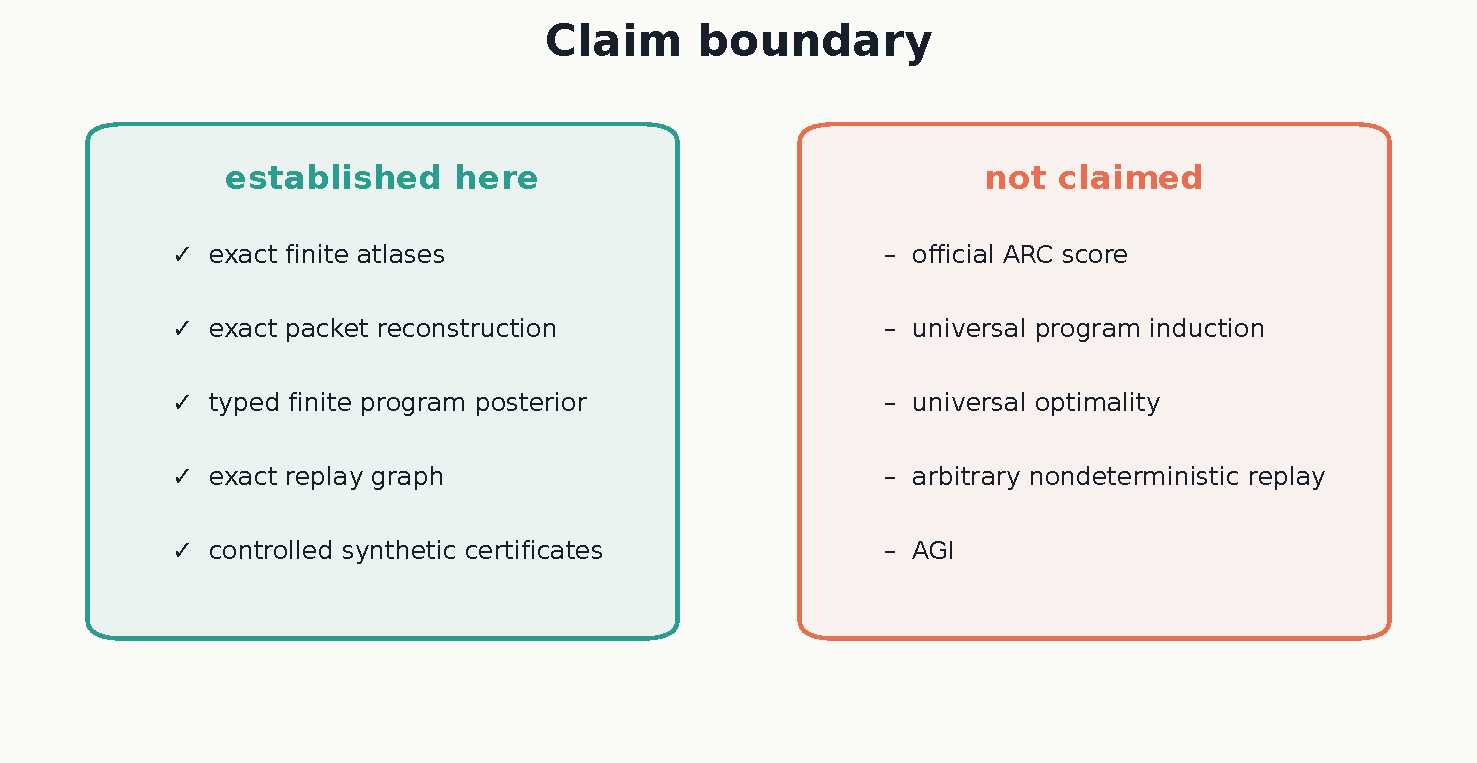
\includegraphics[width=.94\linewidth]{28_claim_boundary.pdf}
\caption{The proof and benchmark boundary is part of the model specification.}
\end{figure}

\section{What has been completed}

The construction now contains every layer required for one coherent large signal model:
\begin{enumerate}
\item exact multi-atlas observation coordinates;
\item Fourier, Haar-wavelet, polyphase, spatial, and categorical realizations;
\item a normalized redundant reconstruction theorem;
\item named feature groups and nested statistical states;
\item exact adaptive packet-tree refinement;
\item a typed nonlinear and memory-bearing operator grammar;
\item Bayesian evidence and posterior uncertainty;
\item exact transition-graph memory;
\item replay-safe active planning;
\item synthetic mechanism-identification and interactive certificates;
\item a source-blind offline adapter and twenty-five local environment trees;
\item a reproducible package, test suite, figures, tables, and run scripts.
\end{enumerate}

\begin{figure}[H]
\centering
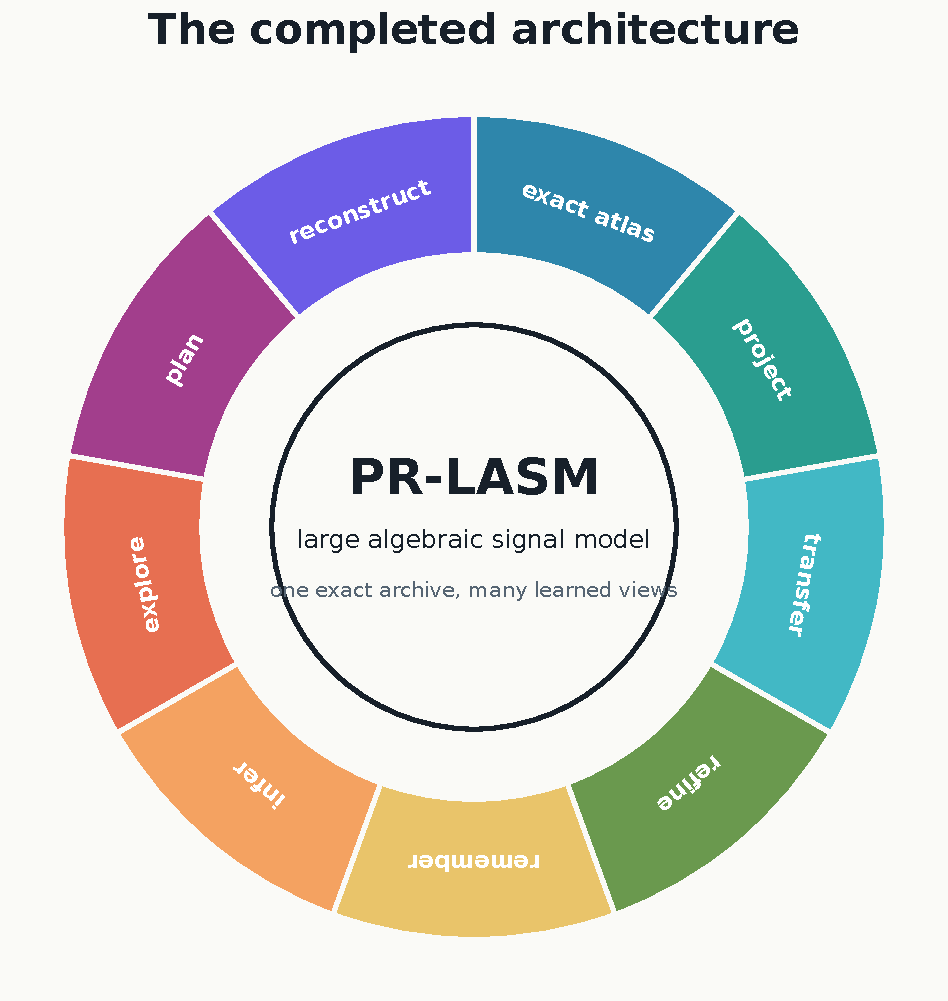
\includegraphics[width=.72\linewidth]{30_closing_wheel.pdf}
\caption{The completed model closes exact analysis, learning, exploration, planning, and reconstruction.}
\end{figure}

\section{Remaining research directions}

The model is finished as a finite architecture, but several extensions are mathematically substantive.

\subsection{Program grammar growth}

A future compiler should be able to propose new typed operator programs while preserving an explicit description length and proof-status boundary.  Arbitrary feature generation would destroy the meaning of the posterior over mechanisms.

\subsection{Learned invertible atlases}

The present exact atlases are fixed.  One may add learned transforms only when their inverse, conditioning, and packet selectors remain explicit.  A learned bijection without stable synthesis is not an exact atlas in the present sense.

\subsection{Continuous and stochastic worlds}

The finite graph can be replaced by kernels or stochastic transition operators.  Exact replay edges then become probability distributions, and frontier planning requires uncertainty over both the world and the graph itself.

\subsection{Scaling and hardware}

Packet-sparse expert fitting, batched small regressions, structured transforms, and graph-local updates are natural GPU targets.  The present CPU certificates do not establish an optimal hardware design.

\subsection{Empirical evaluation}

The next empirical step is straightforward: install the official local runtime on the target machine, execute the bundled suite, preserve complete traces, and compare PR-LASM against the earlier Bayesian operator runner and graph-only ablations under identical budgets.  That is an experiment, not another missing architectural component.

\section{Conclusion}

PR-LASM treats a signal world as more than a stream of vectors.  An observation has several exact coordinate descriptions; an operator has packet transfer blocks; nonlinear behavior has interaction features; memory has typed kernels; uncertainty lives over mechanisms and representations; exploration creates an exact graph where possible; and every compression remains attached to an exact reconstruction archive.

The result is not a language model disguised as a signal model, and it is not a dense predictor decorated with wavelets after the fact.  It is an algebraic production system:
\begin{center}
\fbox{\begin{minipage}{0.91\linewidth}
\centering
\textbf{signal object}
$\to$
\textbf{exact atlas portfolio}
$\to$
\textbf{packet features and nested states}
$\to$
\textbf{typed operator posterior}\\[4pt]
$\to$
\textbf{memory and transition graph}
$\to$
\textbf{active action}
$\to$
\textbf{residual}
$\to$
\textbf{selective refinement}
$\to$
\textbf{exact reconstruction}
\end{minipage}}
\end{center}
Within its finite declared scope, that loop is complete.

\appendix
\clearpage
\section{Exact transform formulas}

\subsection{Haar analysis and synthesis}
For one pair,
\[
\ell=\frac{a+b}{\sqrt2},\qquad h=\frac{a-b}{\sqrt2},
\]
and
\[
a=\frac{\ell+h}{\sqrt2},\qquad b=\frac{\ell-h}{\sqrt2}.
\]
Applying these identities separably and recursively proves the finite two-dimensional transform used in the code.

\subsection{Polyphase analysis and synthesis}
For modulus $N$,
\[
(\Acal_Nx)_{r,s}[q,t]=x[Nq+r,Nt+s].
\]
The synthesis operator places each channel value back at its unique original address.  Therefore
\[
\Scal_N\Acal_N=I.
\]

\subsection{Fourier selector projectors}
For any diagonal zero-one mask $E_B$,
\[
P_B=F^*E_BF,
\]
so
\[
P_B^2=P_B,\qquad P_B^*=P_B.
\]
Disjoint masks annihilate, and a complete mask partition sums to the identity.

\section{Bayesian regression formulas}

For one output $y$ and design matrix $X$, take
\[
\beta\mid\sigma^2\sim N(0,\sigma^2\Lambda_0^{-1}),
\qquad
\sigma^2\sim\operatorname{InvGamma}(a_0,b_0).
\]
Then
\[
\Lambda_n=\Lambda_0+X^\top X,
\qquad
\mu_n=\Lambda_n^{-1}X^\top y,
\]
\[
a_n=a_0+\frac n2,
\qquad
b_n=b_0+\frac12(y^\top y-\mu_n^\top\Lambda_n\mu_n).
\]
For a feature row $x_*$, the predictive mean is $x_*^\top\mu_n$ and the Student predictive scale contains
\[
1+x_*^\top\Lambda_n^{-1}x_*.
\]
The implementation applies this independently to every output coordinate while sharing the design covariance.

\section{Reproducibility commands}

\subsection{Linux or macOS shell}
\begin{lstlisting}
cd Komorebi_PR_LASM_Ultimate
export PYTHONPATH="$PWD/src"
pytest -q
python -m komorebi_arc3_offline.lasm_cli benchmark \
  --output results/pr_lasm_benchmark
\end{lstlisting}

\subsection{PowerShell}
\begin{lstlisting}
$Work = "$env:USERPROFILE\Downloads\Komorebi_PR_LASM_Ultimate"
Set-Location $Work
$env:PYTHONPATH = "$Work\src"
python -m pytest -q
& "$Work\Run_PR_LASM_Benchmark.ps1"
& "$Work\Run_PR_LASM_Smoke.ps1"
\end{lstlisting}

\subsection{Local twenty-five-environment run}
\begin{lstlisting}
& "$Work\Run_PR_LASM_5_Easiest.ps1" -EnvName "arc3-offline"
& "$Work\Run_PR_LASM_All_25.ps1" -EnvName "arc3-offline"
\end{lstlisting}

\section{Machine-readable result files}

The benchmark directory contains:
\begin{itemize}
\item \texttt{exactness\_benchmark.json};
\item \texttt{operator\_benchmark.json} and \texttt{operator\_benchmark.csv};
\item \texttt{agent\_benchmark.json} and \texttt{agent\_benchmark.csv};
\item \texttt{benchmark\_summary.json};
\item per-environment traces, posterior traces, graph summaries, and result files.
\end{itemize}

\section{Test map}

\begin{longtable}{L{0.42\linewidth}L{0.49\linewidth}}
\toprule
test group&content\\
\midrule
\endfirsthead
\toprule
test group&content\\
\midrule
\endhead
Inherited offline runner&actions, packetizer, Bayesian model, replay, offline guard, official-adapter contract, CLI, suite discovery, suite bundle\\
Exact atlases&spatial, Fourier, Haar, polyphase, color, weighted tight-frame synthesis\\
Packet projectors&Fourier band completeness, polyphase completeness, wavelet subband completeness\\
Nested packetizer&determinism, dimensions, reconstruction ledger\\
Adaptive basis&mixed-depth selection and exact synthesis\\
Transition graph&frontier paths and winning edges\\
Program posterior&seven parametrized mechanism and atlas identifications\\
Interactive agent&sequence, click, navigation, and phase-switch environments\\
\bottomrule
\end{longtable}

\end{document}
